\documentclass[driverfallback=dvipdfmx,final]{pittetd}

\usewithpatch{graphicx}
\usepackage{amsmath,amsthm}
\usepackage{multicol}
\usepackage{tabularx}
\usepackage{fixltx2e}
\usepackage{url}
\usepackage{color}
\usepackage{wrapfigure}
\usepackage{amssymb}
\usepackage{epsfig}
\usepackage{subfigure}

%\usepackage{subcaption}
%\usepackage[labelformat=simple,font=footnotesize]{subcaption}
\usepackage[font=small,labelfont=bf]{caption}

\usepackage[square, authoryear]{natbib}
% ADD THE FOLLOWING COUPLE LINES INTO YOUR PREAMBLE
\let\OLDthebibliography\thebibliography
\renewcommand\thebibliography[1]{
  \OLDthebibliography{#1}
  \setlength{\parskip}{0pt}
   \setlength{\bibsep}{0ex} %% vertical spacing between references
  \setlength{\itemsep}{7pt plus 0.3ex} %%
}
\newtheorem{theorem}{Theorem}
\newtheorem{corollary}{Corollary}[theorem]
\renewcommand\thesubfigure{(\alph{subfigure})}
\usepackage{soul}
\usepackage{footnote}
\usepackage{pifont}
\usepackage{chngcntr}
\counterwithin{figure}{chapter}
\counterwithin{table}{chapter}
%\usepackage[nottoc]{tocbibind}

%\usepackage{tikz}
%\usetikzlibrary{fit,positioning}

\let\citeN\citet
\let\cite\citep

\patch{amsmatch}
\patch{amsthm}
\title[Adaptive and Power-aware Fault Tolerance for Future Extreme-scale Computing]
{Adaptive and Power-aware Fault Tolerance for Future Extreme-scale Computing}
\author{Xiaolong Cui}
\degree{Bachelor of Engineering \\ Xi'an Jiaotong University \\2012}
%\date{July 20th 1967} % This date is the date of the thesis defense. Default is \today
%\year{1967}   % pittetd will use the current year unless otherwise indicated. So this command is not necessary.
\keywords{\LaTeX, pittetd, theses, format}   % default, don't change
\subject{Entity/Event-Level Sentiment Detection and Inference} %This fills in the 'Subject' field in Acrobat Reader's Document Info dialog box.
\school{Kenneth P. Dietrich School of \\ Arts and Sciences} %The name of the school will be preceeded by 'the' unless otherwise specified, as in:
%\school[certain]{department}
%
%\chapterfloats%                    Un-comment this to get figures and tables numbered within chapters.
\begin{document}
\maketitle
%
% For the committee membership page, you have to provide the names and affiliations of the members. The first one will 
% be treated by pittetd as the committee chair (thesis/dissertation advisor).
\committeemember{Dr. Taieb Znati, Department of Computer Science, with joint appointment in Telecommunication Program, University of Pittsburgh}
\coadvisor{Co-advisor: Dr. Rami Melhem, Department of Computer Science, University of Pittsburgh}%         This is used if there are two advisors.
\committeemember{Dr. Rami Melhem, Department of Computer Science, University of Pittsburgh}%         This is used if there are two advisors.
\committeemember{Dr. John Lange, Department of Computer Science, University of Pittsburgh}
\committeemember{Dr. Esteban Meneses, School of Computing, Costa Rica Institute of Technology} 
% etc., as many as needed. For master's theses, the committee may be omitted, naming only the advisor.
\school{Computer Science Department}
\makecommittee
\copyrightpage                     %Uncomment this to get a copyright page.
\begin{abstract}
As the demand for computing power continue to increase, both HPC community and Cloud service provides are building larger computing platforms to take advantage of the power and economies of scale. On the HPC side, %several of the most powerful countries are competing for developing the next generation supercomputer--exascale computing machines 
a race is underway to build the world's first exascale supercomputer 
to accelerate scientific discoveries, big data analytics, etc. On the Cloud side, major IT companies are all expanding large-scale datacenters, for both private usage and public services. However, aside from the benefits, several daunting challenges will appear when it comes to extreme-scale.

This thesis aims at simultaneously solving two major challenges, i.e., power consumption and fault tolerance, for future extreme-scale computing systems. We come up with a novel power-aware computational model, referred to as Lazy Shadowing, to achieve high-levels of resilience in extreme-scale and failure-prone computing environments. Different approaches have been studied to apply this model. Accordingly, precise analytical models and optimization framework have been developed to quantify and optimize the performance, respectively. 

In this work, I propose to continue the research in two aspects. Firstly, I propose to develop a MPI-based prototype to validate Lazy Shadowing in real environment. Using the prototype, I will run benchmarks and real applications to measure its performance and compare to state-of-the-art approaches. Then, I propose to further explore the adaptivity of Lazy Shadowing and improve its efficiency. Based on the specific system configuration, application characteristics, and QoS requirement, I will study 
the impact of process mapping the viability of partial shadowing.     

\end{abstract}
% If you say \begin{abstract}[Keywords:] instead of the simple \begin{abstract}, a list of the keywords is appended.
% The list comes from the \keywords command above.
% The starred version \begin{abstract*} typesets the word `ABSTRACT' on the top of the page


\tableofcontents
%\listoftables                      %Pittetd will complain if you tell it to create a list of tables when there are no
%                                   tables (as in this sample file). Uncomment this command if you have tables.
%\listoffigures                     %Obvious analogous for figures.
%\preface
% This is the text of the preface, with acknowledgments, dedication, etc. It is optional, and you create, as shown, by 
% just saying \preface and starting the preface's actual text. Note that 'foreword' is no longer acceptable as title
% for this preliminary.
%
%Conventions, such as notation (nomenclature) and abbreviations, don't receive their own preliminary page. They can be included as an appendix, or as part of the introduction.
%
\chapter{INTRODUCTION}
\label{chapter:intro}
As our reliance on IT continues to increase, the complexity and urgency of the problems our society will face 
in the future drives us to build more powerful and accessible computer systems. Among the different types of 
computer systems, High Performance Computing (HPC) and Cloud Computing systems are the two most powerful ones. 
For both, the computing power attributes to the massive amount of parallelism, which is enabled by 
the massive amount of CPU cores, memory modules, communication devices, storage components, etc. 

Since CPU frequency flattened out in early 2000s, parallelism has become the ``golden rule" to boost performance. 
In HPC, Terascale performance was achieved in the late 90’s with fewer than 10,000 heavyweight single-core processors. 
A decade later, petascale performance required about ten times more processors with multiple cores on each processor. Nowadays, a race
is underway to build the world's first exascale machine to accelerate scientific discoveries and breakthroughs. It is 
projected that an exascale machine will achieve billion-way parallelism by using one million sockets each supporting 
1,000 cores~\cite{doe_ascr_exascale_2011,top_ten_2014}. 

Similar trend is happening in Cloud Computing. 
As the demand for Cloud Computing accelerates, cloud service providers  
will be faced with the need to expand their underlying infrastructure to ensure the expected levels of performance, reliability and cost-effectiveness. 
As a result, lots of large-scale data centers have been and are being built by IT companies
to exploit the power and economies of scale. 
For example, Google, Facebook, and Rackspace have hundreds of thousands 
of web servers in dedicated data centers to support their business. 

Unfortunately, several challenging issues come with the increase in system scale. As today's HPC and Cloud Computing systems grow to 
meet tomorrow's compute power demand, the behavior of the systems will be increasingly difficult to specify, predict and manage. 
This upward trend, in terms of scale and complexity, has a direct negative effect on the overall system reliability. 
%Even with the expected improvement in the reliability of future computing technology, the rate of system level failures will 
%dramatically increase with the number of components, possibly by several orders of magnitude. 
At the same time, the rapid 
growing power consumption, as a result of the increase in system components, is another major concern. 
%It is reported that 
%the power required to run the machines as well as cool them has become the largest cost factor in a large-scale system's operating 
%expenses.  
At future extreme-scale, failure would become a norm rather than an exception, 
driving the system to significantly lower efficiency with unprecedented amount of power consumption. 

\section{Problem Statement}

The system scale needed to address our future computing needs will come at the cost of increasing complexity, unpredictability, 
and operating expenses. As we approach future extreme-scale computing, two of the biggest challenges will be system resilience and power 
consumption, both being direct consequences of the dramatic increase in the number of system components~\cite{exa_challenge_2010,snir2014addressing}. 

Regardless of the reliability of individual component, the system level failure rate will continue to increase as the number of 
components increases, possibly by several orders of magnitude. It is projected that the Mean Time Between Failures (MTBF) of future extreme-scale systems will be at the order of hours or even minutes, meaning 
that many failures will occur every day~\cite{Bergman08exascalecomputing}. Without an efficient fault tolerance mechanism, faults will be so frequent that the applications running on the 
systems will be continuously interrupted, requiring the execution to be restarted every time there is a failure. 

Also thanks to the continuous growth in system components, there has been a steady rise in power consumption in large-scale distributed systems. 
In 2005, the peak power consumption of a single supercomputer reached 3.2 Megawatts. This number was doubled only after 5 years, and reached 17.8 
Megawatts with a machine of 3,120,000 cores in 2013. Recognizing this rapid upward trend, the U.S. Department of Energy has set 20 
megawatts as the power limit for future exascale systems, 
challenging the research community to provide a 1000x improvement in performance with only a 10x increase in power~\cite{exa_challenge_2010}. 
This huge imbalance makes system power a leading design constraint on the path to exascale. 

Today, two approaches exist for fault tolerance. The first approach is rollback recovery, which rolls back and restarts the execution 
every time there is a failure. This approach is often equipped with checkpointing to periodically save the execution state to a 
stable storage so that execution can be restarted from a recent checkpoint in the case of a failure~\cite{Elnozahy:02:Survey,kalaiselvi_sadhana_2000,Chandy:1985:DSD:214451.214456}. 
Although checkpointing is the most widely used technique in today's HPC systems, it may not scale to 
future extreme-scale systems~\cite{ferreira_sc_2011,elnozahy_dsc_2004,4367962}. Given the anticipated increase in system level failure rates and the time to checkpoint large-scale 
compute-intensive and data-intensive applications, the time required to periodically checkpoint an application 
and restart its execution will approach the system's MTBF~\cite{Cappello:2009:TER:1640402.1640428}. Consequently, applications will make little forward progress, thereby 
reducing considerably the overall system efficiency. 

The second approach, referred to as process replication, exploits hardware redundancy and executes multiple instances of the same task 
in parallel to overcome failure and guarantee that at least one task instance reaches completion~\cite{bartlett_1981_nonstop,tsai_isads_2011,ferreira_sc_2011}. Although this approach is extensively used 
to deal with failures in 
Cloud Computing and mission critical systems, it has 
never been used in any HPC system due to its low system efficiency. To replicate each process, process replication requires 
at least double the amount of compute nodes, which also increases the power consumption proportionally. 

Based on above analysis, neither of the two approaches is efficient for future extreme-scale systems. And unfortunately, neither 
of them addresses the power cap issue. 
Achieving high resilience to failures under strict power constraints is a daunting and critical challenge that requires new 
computational models with scalability, adaptability, and power-awareness in mind. 
 
\section{Research Overview}

There is a delicate interplay between fault tolerance and power consumption. Checkpointing and process replication require 
additional power to achieve fault tolerance. Conversely, it has been shown that lowering supply voltages, a commonly used 
technique to conserve power, increases the probability of transient faults~\cite{chandra2008defect,zhao2008reliability}. The trade-off between fault free operation and 
optimal power consumption has been explored in the literature~\cite{meneses2014energy,mills2014energy}. Limited insights have emerged, however, with respect to how 
adherence to application's desired QoS requirements affects and is affected by the fault tolerance and power consumption 
dichotomy. In addition, abrupt and unpredictable changes in system behavior may lead to unexpected fluctuations in performance, 
which can be detrimental to applications’ QoS requirements. The inherent instability of extreme-scale computing systems, 
in terms of the envisioned high-rate and diversity of faults, together with the demanding power constraints under which 
these systems will be designed to operate, calls for a 
reconsideration of the fault tolerance problem.

To this end, Mills, Znati, and Melhem have proposed a novel computational model, referred to as Shadow Replication, as a  
power-aware approach to achieve high-levels of resilience through forward progress~\cite{mills_2014_icnc,mills_2014_pdp,mills2014power}. Based on Dynamic Voltage and Frequency Scaling (DVFS)~\cite{Orgerie:2014:STI:2597757.2532637,4658633,LeSueur:2010:DVF:1924920.1924921}, Mills studied the computational model and its performance in terms of completion time and energy consumption in HPC systems. Through the use of analytical models, simulations, and experimentation, Mills demonstrated that Shadow Replication can achieve resilience more efficiently than both checkpointing and traditional replication when power is limited. However, in Mills' work Shadow Replication is limited to the use of DVFS, which has been shown to have multiple issues that question its viability~\cite{Eyerman:2011:FDU:1952998.1952999,Keller:EECS-2015-257,chandra2008defect,zhao2008reliability}. In addition, Mills' study is limited to HPC systems and focuses exclusively on minimizing energy consumption with constraints on time to completion. In contrast, QoS requirements for various computing systems can be expressed in multiple dimensions that go beyond time and energy. At the same time, an implementation is needed to verify the computational model both with and without failures. 


%In this thesis, our research objective is to simultaneously address the power and resilience challenges for future extreme-scale 
%systems so that both system efficiency and application QoS are guaranteed.
%To this end, we propose an adaptive and power-aware computational model, referred to as Lazy Shadowing, as an efficient and 
%scalable alternative to achieve high-levels of resilience, through forward progress, in extreme-scale, failure-prone 
%computing environments. 
%The basic tenet of Lazy Shadowing is to associate with each main process a suite of “shadows” whose size depends on the 
%``criticality" of the application and its performance requirements. Each shadow process is an exact replica of the original 
%main process. To tolerate failures, the main process and its associated shadow processes will execute in parallel, but on 
%different compute nodes. 
%The shadows initially execute at a reduced rate %via Dynamic Voltage Frequency and Scaling (DVFS) 
%to save power. 
%If the main process completes the task successfully, we will 
%terminate the shadows immediately. If the main process fails, however, we will promote one of the shadow processes to be a 
%new main process and possibly increase its execution rate to mitigate delay.

To address the above limitations, this thesis builds on the computational model of Shadow Replication, and seeks to simultaneously address the power and resilience challenges for future extreme-scale systems while guaranteeing system efficiency and application QoS.
Specifically, this thesis tries to answer 4 questions: 1) is Shadow Replication general enough to achieve objectives beyond time to completion; %, such as multiple simultaneous requirements defined in a SLA in the Cloud; 
2) how to enable Shadow Replication when DVFS is not viable, and ensure forward progress in failure-prone, extreme-scale systems; 3) is the computational model realistic in real environments; and 4) how to make the computational model reflective of the propensity of the processing elements to failures and adaptive to different environments and requirements.
With these questions in mind, 
I have studied different techniques to embody and augment the model, and developed analytical frameworks for different objectives in the Cloud and HPC environments~\cite{cui_2014_closer,cui_en7085151,cui_2016_scalcom}.
%Previously, we have formally defined the computational model, studied possible techniques to realize and optimize the idea, and 
%built analytical models for performance evaluation. 
To complete my thesis, I propose to extend the study in the following two aspects.
Firstly, I propose to implement a prototype in the context of Message Passing Interface (MPI), to validate the 
computational model as well as measure its performance in real environment. Secondly, I propose to study  
``smart shadowing" which adapts to the system configuration, application characteristics, and QoS requirement.
In summary, my thesis will consist of the following main components.

%\subsection{Lazy Shadowing: a novel fault-tolerant computational model (completed)}

%The basic tenet of Lazy Shadowing is to associate with each main process a suite of “shadows” whose size depends on the 
%``criticality" of the application and its performance requirements. Each shadow process is an exact replica of the original 
%main process. To tolerate failures, the main process and its associated shadow processes will execute in parallel, but on 
%different compute nodes. 
%The shadows initially execute at a reduced rate %via Dynamic Voltage Frequency and Scaling (DVFS) 
%to save power. 
%If the main process completes the task successfully, we will 
%terminate the shadows immediately. If the main process fails, however, we will promote one of the shadow processes to be a 
%new main process and possibly increase its execution rate to mitigate delay. This continues until the task completes. 

%Given that the failure rate of an individual node is much lower than the aggregate system failure, it is very likely that 
%the main process will always complete its execution successfully, thereby achieving fault tolerance at a significantly reduced 
%cost of power. Consequently, the high probability that shadows never have to complete the full task, coupled with the fact that 
%they initially only consume a minimal amount of power, dramatically increases a power-constrained system's tolerance to failure.

\subsection{Reward-based optimal Shadow Replication (completed)}
Shadow Replication is a flexible computational model that can achieve multi-dimensional QoS requirements. 
The major challenge resides in determining jointly the execution rates of all task instances, 
both before and after a failure occurs, with the objective to optimize performance, resilience, power consumption, or their combinations.
In this work we focus on the Service Level Agreement (SLA) requirements in the Cloud and develop a reward-based analytical framework, in order to derive the optimal execution rates for maximizing reward and minimizing energy 
costs under strict completion time constraints~\cite{cui_2014_closer,cui_en7085151}. 

%To define the reward-based analytical framework, we first define a failure model that considers the failure distribution of each process, and a power model that describes the power consumption characteristics under different states. Based on the failure model and power model, we then derive the expected income as a function of completion time, and the expected energy cost as a product of power and time. Lastly, the reward is defined as the optimization objective to balance between completion time and energy cost.  



\subsection{Lazy Shadowing (completed)}

Enabling Shadow Replication for resiliency in extreme-scale computing brings about a number of challenges and design decisions, including the applicability of this concept to a large number of tasks executing in parallel, 
the effective way to control shadows’ execution rates, and the runtime mechanisms and communications support to ensure efficient 
coordination between a main and its shadow. Taking into consideration the main characteristics of compute-intensive and 
highly-scalable applications, 
we devise novel ideas of shadow collocation and shadow leaping, and integrate them with Shadow Replication to form a more efficient and scalable paradigm that we call Lazy Shadowing~\cite{cui_2016_scalcom}.
%we design two novel techniques, referred to as shadow collocation and shadow leaping, 
%in order to achieve high tolerance to failures while minimizing delay and power consumption.

%To control the processes' execution rate, DVFS can be applied while each process resides on one core exclusively. 
%The effectiveness of DVFS, however, may be markedly 
%limited by the granularity of voltage control, the number of frequencies available, and the negative effects on 
%reliability. 
%An alternative is to collocate multiple processes on each core while keeping all the cores executing at maximum frequency. 
%Then time sharing can be used to achieve the desired execution rates for each collocated process. 
%Since this approach collocates multiple processes on a core, it simultaneously reduces the number of compute nodes and 
%the power consumption. 
%
%Furthermore, we identify a unique opportunity that ensures forward progress in failure-prone environments. Since each shadow process is associated with a main process, the lagging shadow can benefit from the faster execution 
%of the main with minimal overhead. Specifically, when a failure occurs, Lazy Shadowing takes advantage of 
%the recovery time and leaps forward each shadow by copying states from its associated main. This technique not only achieves forward 
%progress for the shadow processes at minimized power and delay, but also reduces the recovery time after each failure.

\subsection{lsMPI: an implementation in MPI (in progress)}

Though Lazy Shadowing has been evaluated analytically, a real implementation 
is necessary for validation and performance measurement in real systems. I am implementing a prototype of Lazy 
Shadowing as a runtime for Message Passing Interface (MPI). %, which is the de facto programming paradigm for HPC. 
%Instead of 
%a full-feature MPI implementation, the runtime is designed to be a separate layer between MPI and user application, in order 
%to take advantage of existing MPI performance optimizations that numerous researches have spent years on. 
The runtime will spawn 
the shadow processes at initialization phase, manage the coordination between main and shadow processes, 
and guarantee order and consistency for messages and non-deterministic events. With this implementation, we will perform thorough 
experiments to measure its runtime overhead as well as performance under failures.

\subsection{Smart shadowing (future)}
Lazy Shadowing is a flexible and adaptive computational model that deserves further investigation. Previous studies have shown that 
different nodes tend to have different failure probabilities, e.g., 19\% of the nodes account for 92\% of the machine check errors on Blue Waters~\cite{di2014lessons}. The reason 
is complicated and may attribute to the manufacture process, heterogeneous architecture, environment factors (e.g. temperature), 
and/or workloads. % I propose to apply machine learning techniques to learn the heterogeneity in failure distributions among a given 
%system's nodes. 
Under differernt failure distribution assumptions, I will study how the mapping from processes to physical cores can impact the performance and cost dichotomy. 
In addition, I will further consider allocating different number of shadow processes for different tasks to reduce cost while 
maintaining performance. 

\section{Contributions}
When completed, this thesis will make the following contributions:

\begin{itemize}
\item A reward-based framework for Shadow Replication to satisfy SLA requirements as well as maximize profit in Cloud Computing
\item Study of Lazy Shadowing as an enhanced model for future extreme-scale systems
\item A fully functional implementation of Lazy Shadowing for Message Passing Interface
\item Exploration of Lazy Shadowing's adaptivity to different environments, workloads, and QoS requirements. 
\end{itemize}


\section{OUTLINE}
\label{outline}
The rest of this proposal is organized as follow:  
Chapter \ref{chapter:background} reviews existing fault tolerance techniques in large-scale distributed systems, 
and Chapter \ref{chapter:shadowing} introduces the Shadow Replication computational model. In Chapter \ref{chapter:reward} we build a reward-based optimization framework for Shadow Replication in the Cloud environment.
In Chapter \ref{chapter:scale}, we introduce Lazy Shadowing which enhances Shadow Replication for extreme-scale systems. 
Implementation issues are discussed in Chapter \ref{chapter:implementation}. Adaptivity and smart shadowing are discussed in Chapter \ref{chapter:smart}.
%Chapter \ref{chapter:timeline} and \ref{chapter:summary} lists the timeline and concludes the proposal, respectively.
Chapter~\ref{chapter:summary}  concludes the proposal.










\chapter{BACKGROUND}
\label{chapter:background}
%Extreme-scale computing presents some unique challenges to fault tolerance as faults are no longer 
%an exceptional event \cite{ferreira_sc_2011}. 
Rollback recovery is the dominant mechanism to achieve fault
tolerance in current HPC environments~\cite{Elnozahy:02:Survey}. In the most general form, rollback recovery 
involves the periodic saving of the execution state (checkpoint), with the anticipation that
in the case of a failure, computation can be restarted from a previously saved checkpoint. % \cite{Elnozahy:02:Survey}. %The identification of an error, before or during a checkpoint,
%requires that the application rollback to the previously completed checkpoint. 
Coordinated checkpointing is a popular approach for
its ease of implementation.
Specifically, all processes
coordinate with one another to produce individual states that satisfy the ``happens before"
communication relationship \cite{chandy_trans_1972}, which is proved to provide a consistent global state.
%Essentially, the algorithm provides a method for all processes involved to stop operation ``at the same
%time" and transfer their system state to a stable storage. 
The major benefit of coordinated checkpointing stems from its simplicity and ease of implementation. 
Its major drawback, however, is the lack of scalability, as it requires global coordination
~\cite{elnozahy_dsc_2004,riesen_sandia_2010}.
%hargrove2006berkeley}.


In uncoordinated checkpointing, processes checkpoint their states independently and postpone creating a 
globally consistent view until the recovery phase. The major advantage is the reduced overhead during fault free operation. However, the scheme requires that
each process maintains multiple checkpoints %and message logs, necessary to construct a consistent 
%state during recovery. It 
and can also suffer the well-known domino effect 
 \cite{randell_domino_effect,alvisi_ftc_1999,helary_rds_1997}. One hybrid approach, known as communication induced 
checkpointing, aims at reducing coordination overhead \cite{alvisi_ftc_1999}. The approach, however, may 
cause processes to store useless states. To address this 
shortcoming, ``forced checkpoints" have been proposed \cite{helary_rds_1997}. This approach, however,  may lead to unpredictable
checkpointing rates. 
Although well-explored, uncoordinated checkpointing has not been widely adopted
in HPC environments for its complexities. 
%its dependency on applications \cite{guermouche_2011_ipdps}.


One of the largest overheads in any checkpointing process is the time necessary to write the checkpointing 
to stable storage. Incremental checkpointing attempts
to address this by only writing the changes since previous checkpoint \cite{Agarwal:04:Adaptive,elnozahy_1992_manetho,li_trans_1994}. 
This can be achieved using dirty-bit page flags \cite{plank_ftcs_1994,elnozahy_1992_manetho}. Hash based incremental checkpointing, on the other hand, makes use of hashes to detect changes \cite{nam_ftc_1997,Agarwal:04:Adaptive}. 
Another proposed scheme, known as in-memory checkpointing, minimizes the overhead of disk access~\cite{zheng_2004_ftccharm,6264677}.
%offloads the checkpointing process to a secondary task and only writes incremental checkpoints \cite{li_trans_1994}.
The main concern of these techniques is the increase in
memory requirement to support the simultaneous execution of the checkpointing and the application. 
It has been suggested that nodes in extreme-scale systems should be configured with fast local storage~\cite{doe_ascr_exascale_2011}. 
%, which
%improves the performance of checkpointing \cite{doe_ascr_exascale_2011}. 
Multi-level checkpointing , which consists of
writing checkpoints to multiple storage targets, 
can benefit from such a strategy \cite{Moody:10:SCR}. This,
however, may lead to increased failure rates of individual nodes and complicate the checkpoint writing process.
%Furthermore, it may complicate the checkpoint writing process and requires that the system track the
%current location of all process's checkpoints.


Process replication, or state machine replication, has long been used for reliability and availability in distributed and mission critical systems \cite{schneider_1990_tutorial}. %Replication can be used to detect and correct system failures that are otherwise undetectable,
%such as silent data corruption and Byzantine faults \cite{fiala_2012_sdc}. 
%This approach is barely used in HPC systems, primarily due to its low efficiency.
%However, upcoming extreme-scale systems are expected to 
%require a more challenging level of fault tolerance to deal with the 
%confront a dramatic growth in both the frequency and diversity of faults.
%As a result,
Although it is initially rejected in HPC communities, 
replication has recently been proposed to address the deficiencies of checkpointing for upcoming extreme-scale systems \cite{Cappello:09:Fault,engelmann2011redundant}. 
Full and partial
process replication have also been studied to augment existing checkpointing techniques, and to  
detect and correct silent data corruption \cite{stearly_2012_partial,elliott_2012_cpr,ferreira_sc_2011,fiala_2012_sdc}. % There are several different implementations of
%replication in the widely used MPI library, each with their different tradeoffs and overheads. The
%overhead can be negligible or up to 70\% depending upon the communication patterns of the
%application \cite{engelmann2011redundant}. %Moreover, replication alone is not enough to guarantee fault tolerance since
%it is possible that all nodes executing a given process could fail simultaneously, thus
%replication is typically paired with some form of checkpointing. 
Our approach is largely different from classical process replication in that we dynamically configure the execution rates of main and shadow processes, so that less resource/energy is required while reliability is still assured.  


Replication with dynamic execution rate is also explored in Simultaneous and Redundantly Threaded (SRT) processor whereby one leading thread is running ahead of trailing threads \cite{reinhardt2000transient}. However, 
the focus of \cite{reinhardt2000transient} is on transient faults within CPU while we aim at tolerating both permanent and transient faults across all system components.
%Also, this work differs from \cite{mills_2014_icnc,cui_en7085151,cui_2014_closer}, where shadowing with DVFS is studied for single or loosely-coupled tasks. %Instead, in this paper we explore novel ideas of shadow collocation and shadow leaping in order to satisfy the requirements of future extreme-scale HPC systems. 
%our approach is different in that it tunes the execution rates of the leading and trailing threads in a finer grain, in order to achieve a ``parameterized" trade-off between completion time and energy consumption. 
%Further, we take advantage of the idle time during failure recovery and ``leap" the trailing replicas to achieve forward progress%, largely improving performance in terms of both completion time and energy consumption. 
%. This differs from \cite{reinhardt2000transient}, of which the ``leaping" of the trailing replica results in extra overhead.
%To the best of our knowledge,
%Lazy Shadowing is the first attempt to explore a state-machine replication based framework
%that achieves a fine-grained tradeoff between time and hardware redundancy while meeting resilience and
%power requirements.

\chapter{Lazy Shadowing: a novel fault-tolerant computational model}
\label{chapter:shadowing}
%It is without doubt that our understanding of how to build reliable systems out of unreliable components has led the development of robust and fairly reliable large-scale software and networking systems. The inherent instability of extreme-scale distributed systems of the future in terms of the envisioned high-rate and diversity of faults, however, calls for a reconsideration of the fault tolerance problem as a whole. % and the exploration of radically different approaches that go beyond adapting or optimizing well known and proven techniques.

Shadow Replication is a novel computational model that goes beyond adapting or optimizing well known and proven techniques, and explores radically different methodologies to fault tolerance~\cite{mills_2014_icnc,mills_2014_pdp,mills2014power}. % that scale to extreme-scale computing infrastructures. 
%The proposed solutions differ in the type of faults they manage, their design, and the fault tolerance protocols they use. %It is not just a scale up of  ``point" solutions, but an exploration of innovative and scalable fault tolerance frameworks. 
%When integrated, it will lead to efficient solutions for a ``tunable" resiliency that takes into consideration the nature of the data and the requirements of the application.
The basic tenet of Shadow Replication is to associate with each main process a suite of “shadows” whose size depends on the 
``criticality" of the application and its performance requirements. Each shadow process is an exact replica of the original 
main process, 
and a consistency protocol is needed to assure that the main and the shadow are consistent.  
When possible, the shadow executes at a reduced rate to save power.
Shadow Replication achieves power efficiency under QoS requirements by dynamically responding to failures. 
%If the main process completes the task successfully, the associated shadows will be terminated immediately. If the main process fails, however, one of the shadow processes will be promoted to be a 
%new main process, and possibly increase its execution rate to mitigate delay.

Assuming the fail-stop fault model, where a processor stops execution once a fault
occurs and failure can be detected by other processors~\cite{gartner_faults_1999,cristian_comm_1991}, 
the Shadow Replication fault-tolerance model can be described as follows:
\begin{itemize}
	\item A main process, $P_m(W,\text{ }\sigma_m)$, whose responsibility is to executes a task of size $W$ at a speed of $\sigma_m$;
	\item A suite of shadow processes, $P_{s}(W,\text{ }\sigma_b^s, \text{ }\sigma_a^s)$ ($1 \le s \le \cal S)$, where $\cal S$ is the size of the suite. The shadows execute on separate computing nodes. Each shadow process is associated with two execution speeds. All shadows start execution simultaneously with the main process at speed $\sigma_b^s$ ($1 \le s \le \cal S$). Upon failure of the main process, all shadows switch their executions to $\sigma_a^s$, with one shadow being designated as the new main process. This process continues until completion of the task.
\end{itemize}
%All shadows execute simultaneously with the main process at speed $\sigma_a^s$

\begin{figure}[!t]
	\begin{center}
		\subfigure[No Failure]
		{
			\label{fig:sc_no_fail}
			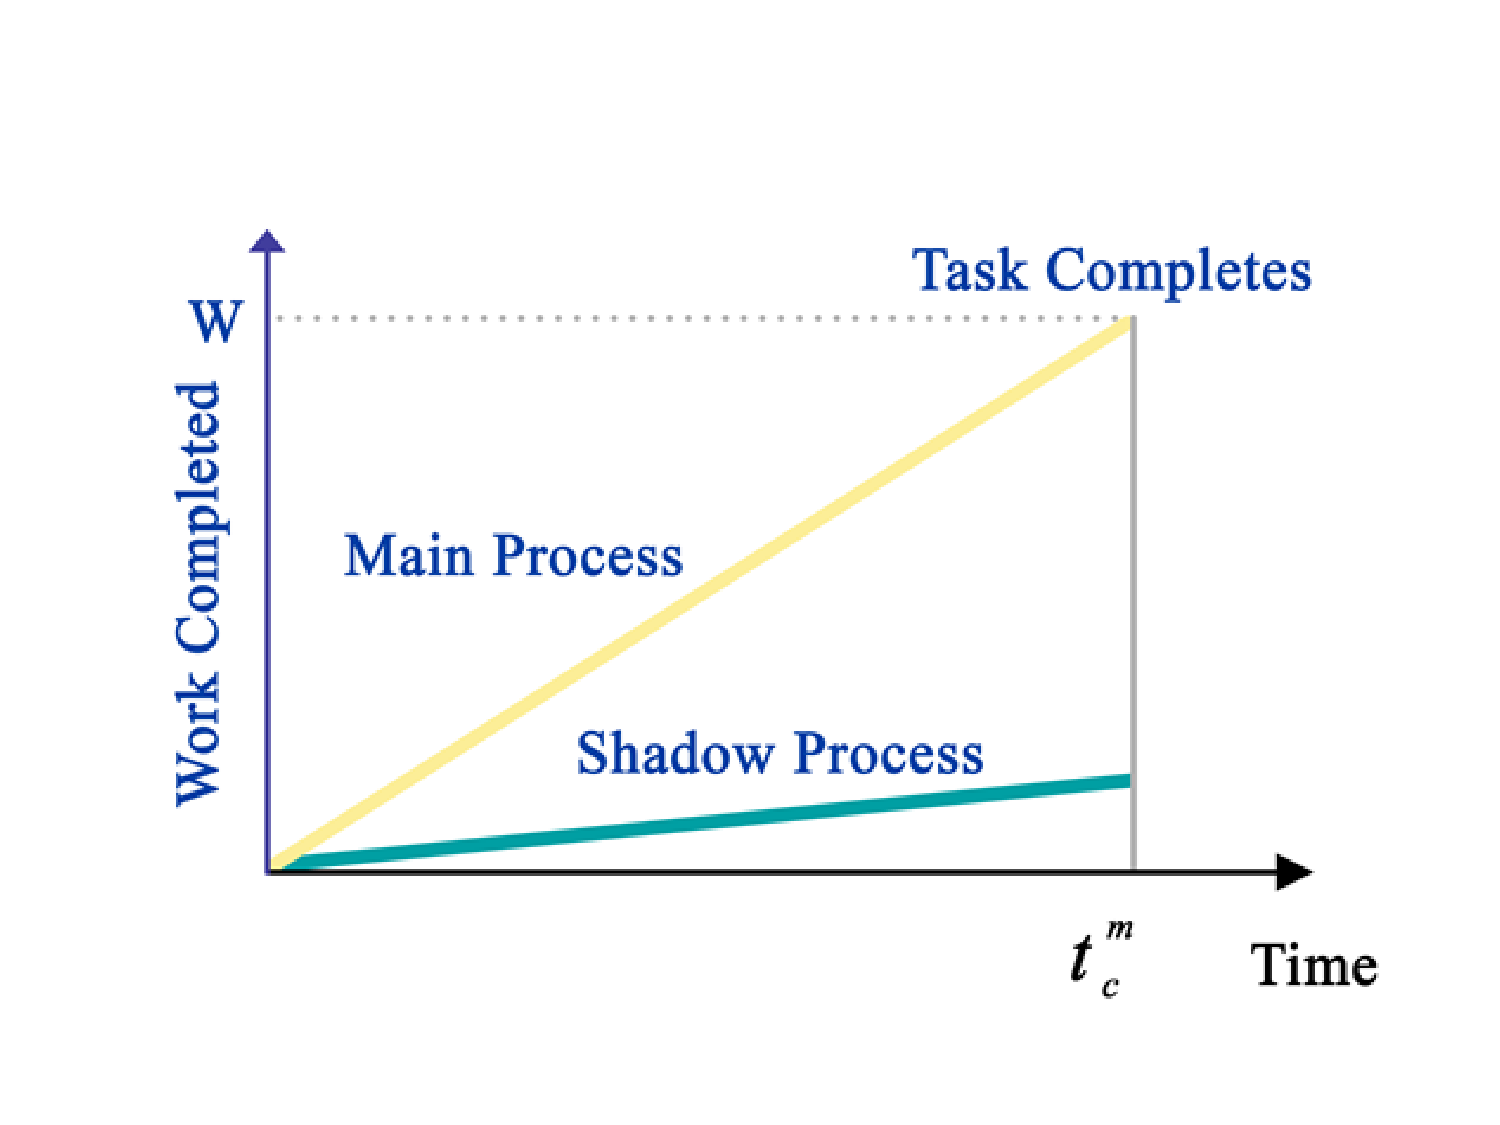
\includegraphics[width=0.31\textwidth]{figures/example1.pdf}
		}
		\subfigure[Shadow Process Failure]
		{
			\label{fig:sc_shadow_fail}
			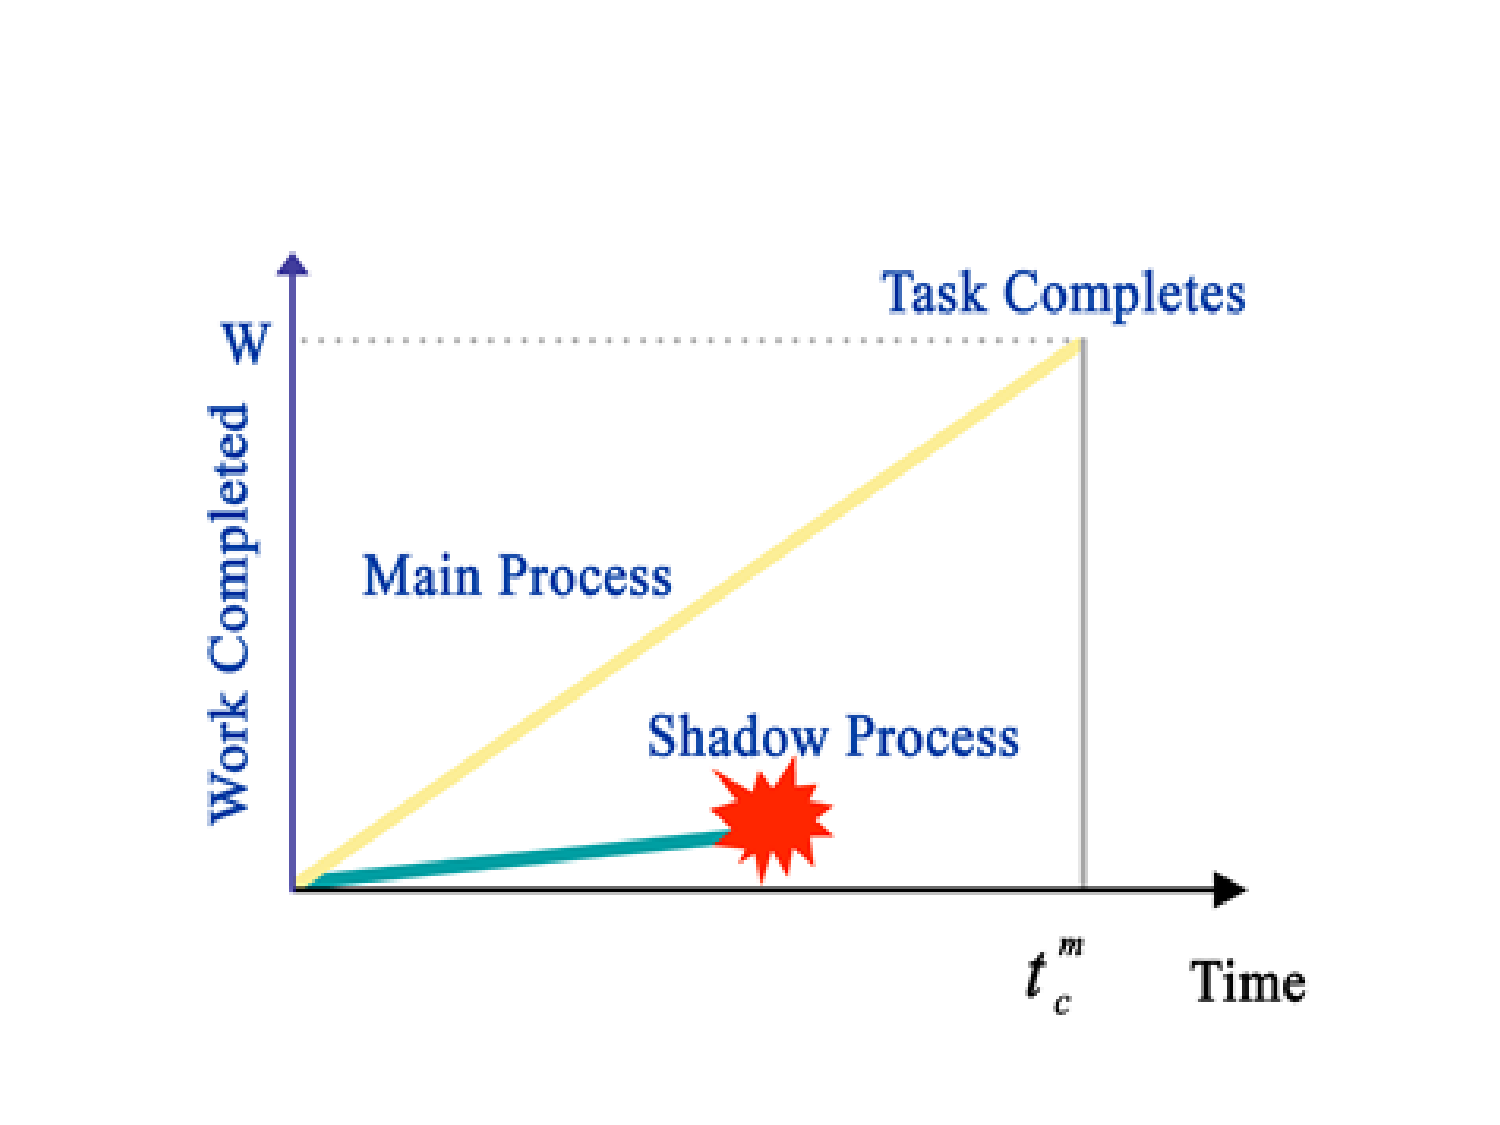
\includegraphics[width=0.28\textwidth]{figures/example3.pdf}
		}
		\subfigure[Main Process Failure]
		{
			\label{fig:sc_main_fail}
			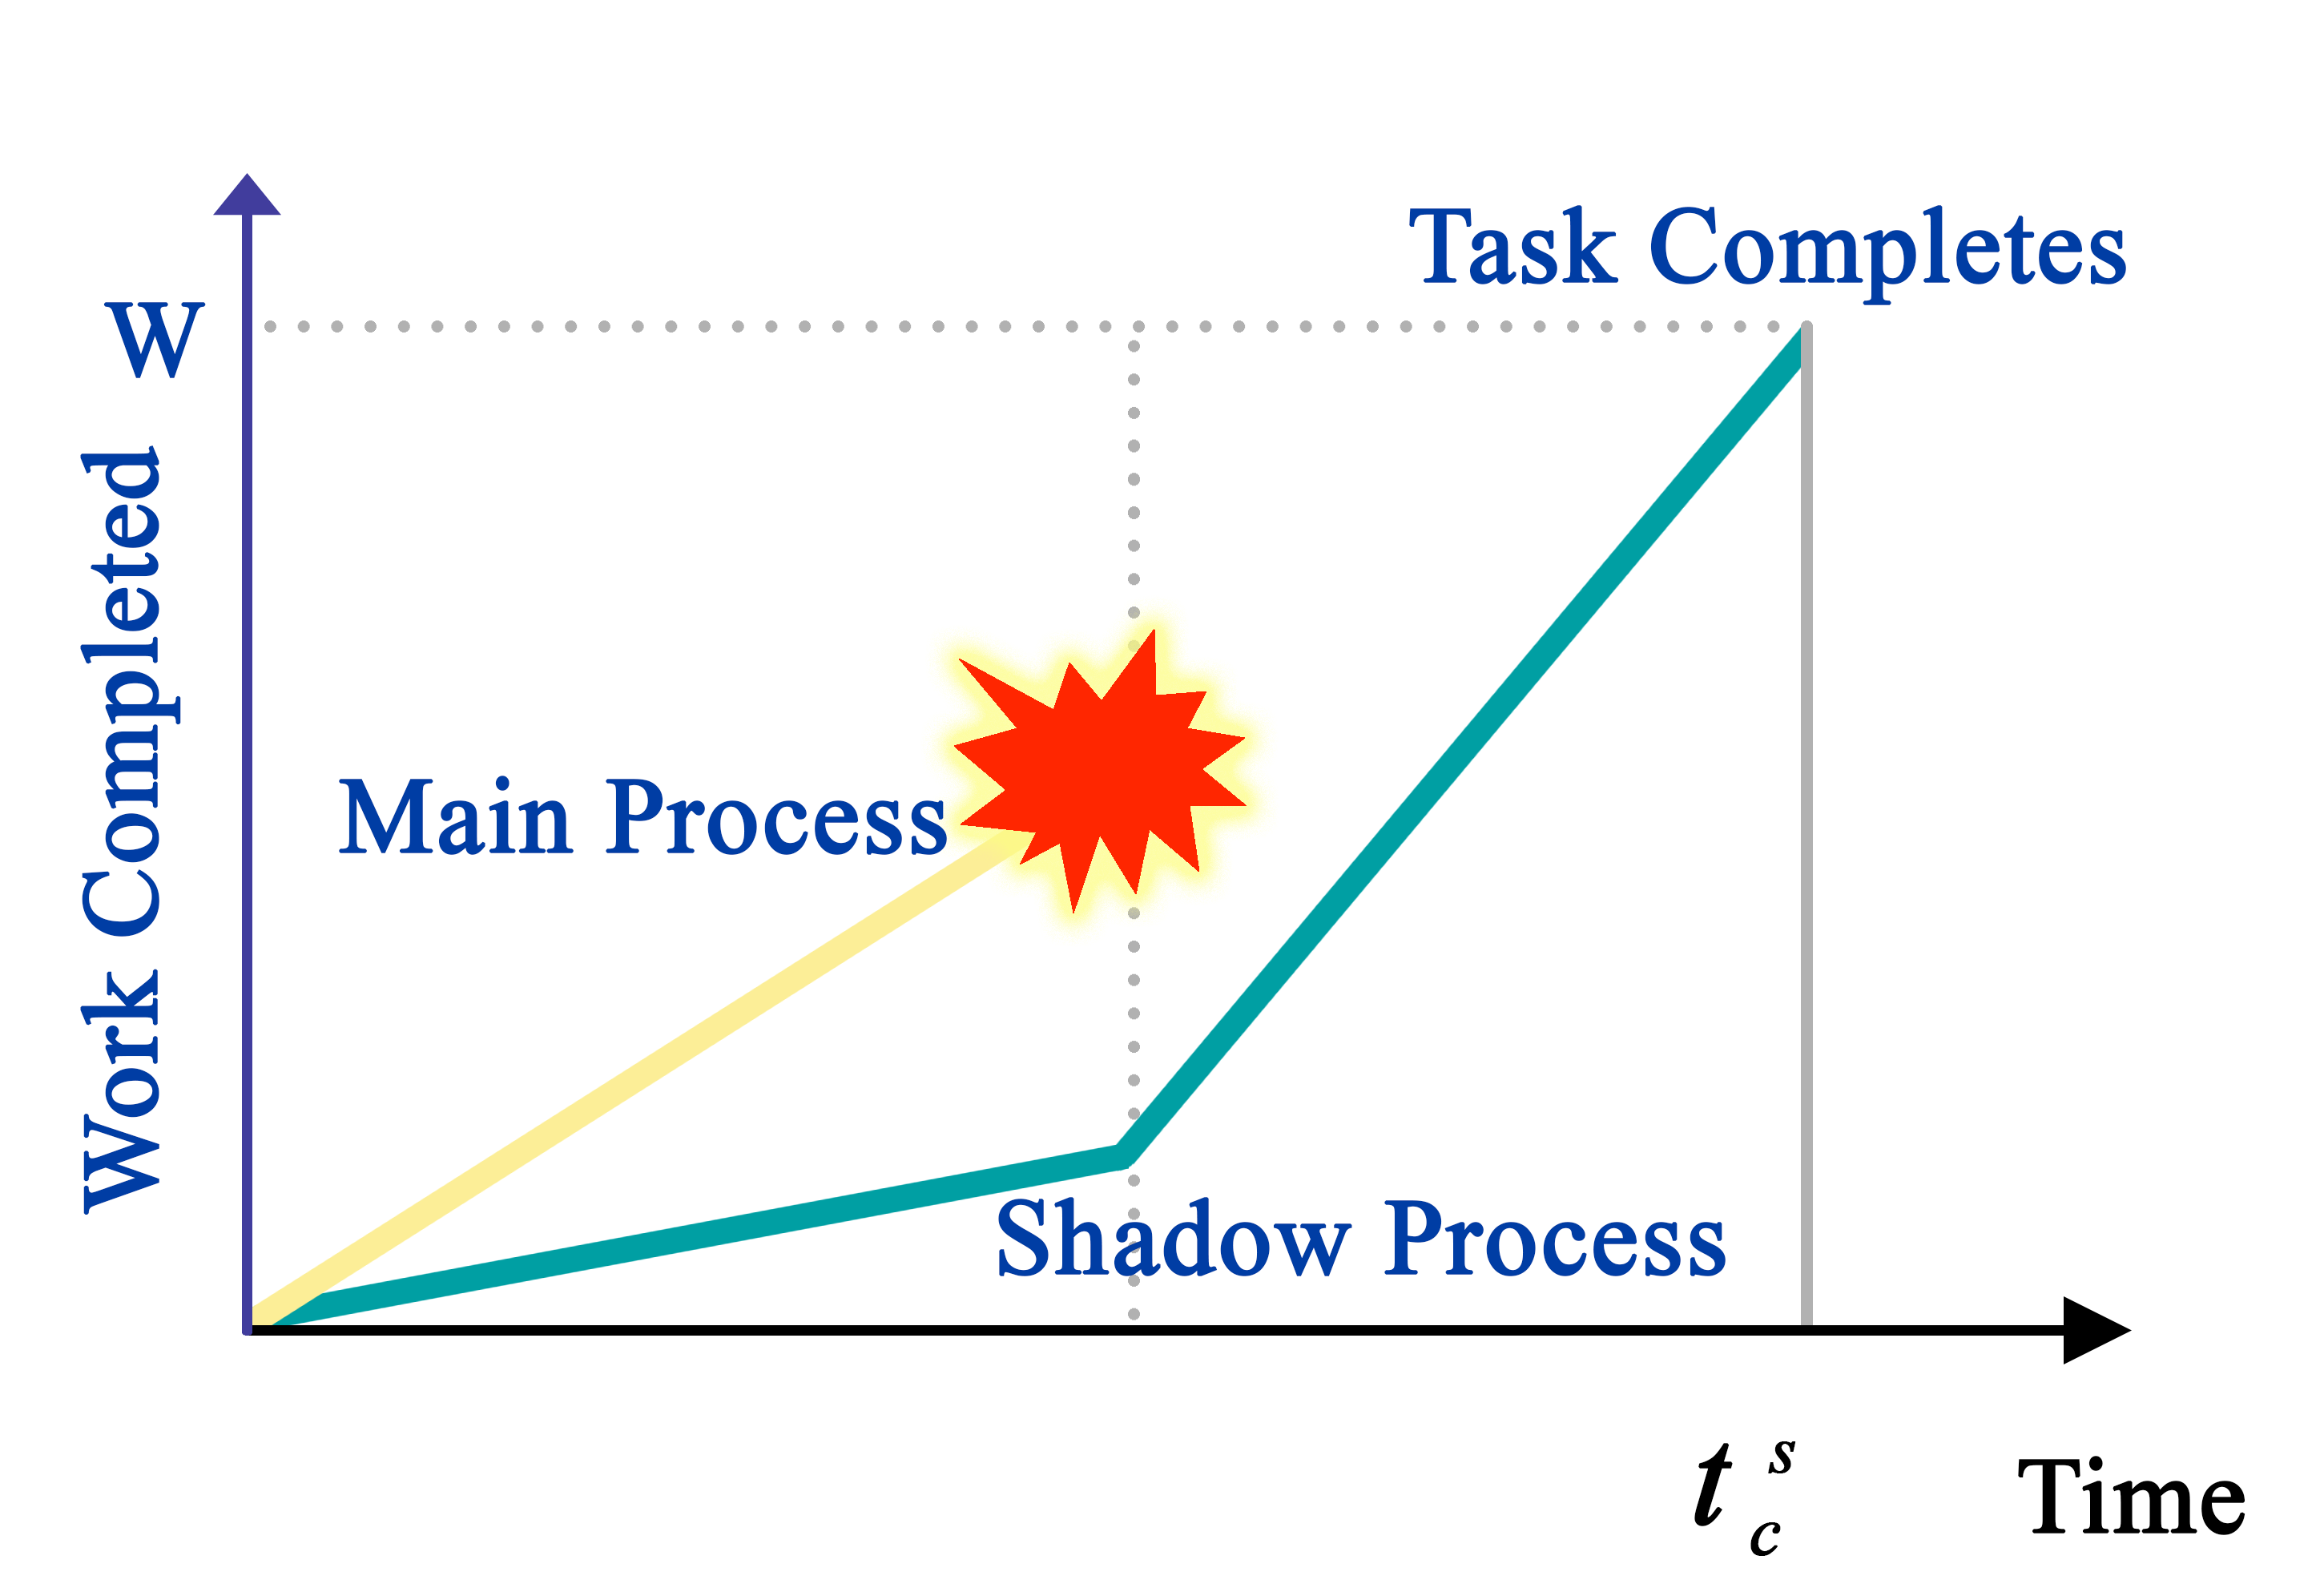
\includegraphics[width=0.32\textwidth]{figures/example2.png}
		}
	\end{center}
	\caption{Shadow Replication for a single task and single replica}
	\label{fig:sc_overview}
\end{figure}

Assuming a single process failure, Figure \ref{fig:sc_overview} illustrates the behavior of Shadow Replication with one shadow per task. 
%To illustrate the behavior of Shadow Replication, we limit the number of shadows to a single process and consider the scenarios depicted in Figure \ref{fig:sc_overview}, assuming a single process failure. 
If the main process does not fail, it will complete the task ahead of its shadow at $t_c^m$. At this time, we terminate the shadow immediately to save power. If the shadow fails before the main completes, the failure has no impact on the progress of the main. If the main fails, however, the shadow switches to a higher speed and completes the task at time $t_c^s$. 
%Figure \ref{fig:sc_no_fail} represents the case when neither the main nor the shadow fails. The main process, executing
%at a higher speed, completes the task at time $t_c^m$. At this time, the shadow process, progressing at a lower speed, stops execution immediately. Figure \ref{fig:sc_shadow_fail} represents the case when the shadow fails. This failure, however, has no impact on the progress of the main process, which still completes the task at $t_c^m$. Figure \ref{fig:sc_main_fail} depicts the case when the main process fails while the shadow is in progress. After detecting the failure of the main process, the shadow begins execution at a higher speed, completing the task at time $t_c^s$. 
Given that the failure rate of an individual node is much lower than
the aggregate system failure, it is very likely that the main process
will always complete its execution successfully, thereby achieving fault tolerance at a significantly reduced cost of energy consumed by the shadow. %saving a lot of energy for its associated shadow processes. 


A closer look at the model reveals that Shadow
Replication is a generalization of traditional fault tolerance
techniques, namely re-execution and process replication. If it allows for flexible completion time, 
Shadow Replication converges to re-execution as
the shadow remains idle during the execution of the main process and
only starts execution upon failure. If the target response time is
stringent, however, Shadow Replication converges to process replication,
as the shadow must execute simultaneously with the main at the same
speed. The flexibility of the Shadow Replication model provides the
basis for the design of a fault tolerance strategy that strikes a
balance between task completion time and energy saving. 

%Given that the probability of two individual nodes executing the same
%instances of a task fail at the same time is low, we will focus on the study of Shadow Replication model with a single shadow. It is clear, however, that the model can
%be extended to support multiple processes, as required by the
%application's fault-tolerance requirement. Furthermore, we adopt the
%fail-stop~ fault model, where a processor stops execution once a fault
%occurs and failure can be detected by other
%processes\cite{gartner_faults_1999,cristian_comm_1991}.

Based on DVFS, Mills studied the computational model in HPC systems and  
demonstrated that Shadow Replication can achieve resilience more efficiently than both checkpointing and process replication when power is limited~\cite{mills_2014_icnc,mills_2014_pdp,mills2014power}.
I am going to extend the work to achieve better flexibility, adaptivity, and scalability. 





\chapter{Reward-based optimal Lazy Shadowing}
\label{chapter:reward}
In the most straightforward form of Shadow Replication, each main is associated with one shadow to tolerate a crash failure, and with two shadows to tolerate a silent failure. 
Similar to traditional process replication, Shadow Replication ensures successful task
completion by running the mains and shadows in parallel. Contrary to process replication, however, Shadow Replication
exploits differential and dynamic execution rates, thereby enabling a
parameterized trade-off between response time, energy consumption and resilience.

After figuring out the shadow suite size according to the fault tolerance requirements, a major challenge resides in determining
jointly the execution rates of all task instances, both before and
after a failure occurs, with the consideration of any objective and any constraint. This chapter addresses the above challenge by formulating it into a generic optimization problem, so that standard and well-known math methods (e.g., quasi-newton) can be naturally applied to solve it and derive the optimal execution rates. With this optimization framework, this chapter also provides a case study in the Cloud with a series of analytical models for failure, power, energy, etc. 

\section{Generic Optimization Framework}
As mentioned in Section~\ref{sec:shadowing_adaptivity}, large-scale computing systems typically aim at maximizing performance, resilience, power/energy consumption, or any of their combination. Given a specific objective, by tuning its execution rates Shadow Replication can be optimized with respect to that objective, while satisfying the provided constraints, if any. A generic optimization framework for this purpose is depicted in Figure~\ref{fig:opt_problem}.

\begin{figure}[t]
	\begin{center}
		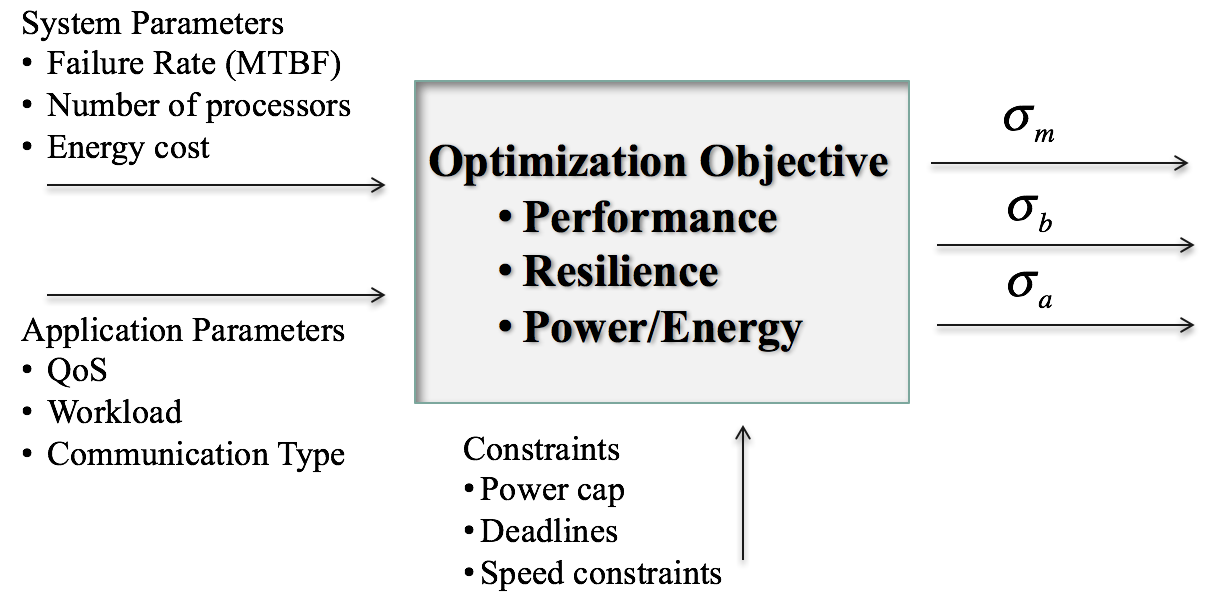
\includegraphics[width=0.9\textwidth]{Figures/opt_problem}
	\end{center}
	\caption{A generic optimization framework for Shadow Replication.}
	\label{fig:opt_problem}
    \vskip -0.1in
\end{figure}

As shown in Figure~\ref{fig:opt_problem}, the inputs to the problem consist of system parameters and application parameters. System parameters include the failure distribution, system scale, and power consumption characteristics. Application parameters could be QoS requirements, total workload, and/or the communication and synchronization patterns. In addition, constraints, such as power cap and deadline, can be specified in observation of resource limitations. Finally, the outputs are the derived execution rates for all processes, which optimize the given objective.

The above optimization framework can be tailored to various computing environments for different needs. For example, in HPC systems, the problem can be simplified by fixing $\sigma_m$ and $\sigma_a$ at the maximum CPU rate and only optimize $\sigma_b$ to minimize energy consumption under deadline constraint~\cite{mills_2014_icnc}. The following section discusses another case study in the Cloud environment that relaxes the constraints on $\sigma_m$ and $\sigma_a$~\cite{cui_2014_closer}. The resulting work, referred to as reward-based optimal Shadow Replication, considers Service Level Agreements (SLA) in the Cloud and optimizes a ``reward'' for Cloud service providers. The flexibility in the definition of reward demonstrates the ability of Shadow Replication to achieve objectives that go beyond time and energy. 



\section{Reward-based Optimal Shadow Replication}
Cloud Computing has emerged as an attractive platform for 
diverse compute- and data-intensive applications, as it allows for
low-entry costs, on demand resource provisioning, and
reduced complexity of maintenance~\cite{tchana_cits_2012}. 
As the demand for cloud computing
accelerates, cloud service providers (CSPs) will be faced with the
need to expand their underlying infrastructure to ensure the expected
levels of performance and cost-effectiveness, resulting
in a multi-fold increase in the number of computing, storage and communication components in their data centers.

Two direct implications of the ever-growing large-scale data centers are the increasing energy costs, which build up the operating expenditure, and service failures, which subject the CSP to a loss of revenue. Therefore, Service Level Agreement (SLA) becomes a critical aspect for a sustainable cloud computing business. 
In its basic form, an SLA is a contract between the CSPs and consumers that specifies the terms and conditions under which the service is to be provided, including expected response time and reliability.


To understand the question of how
fault tolerance might impact power consumption and ultimately the expected profit of CSPs, this section studies the application of Shadow Replication to satisfying SLA requirements in the presence of crash failures in Cloud computing. The rest of the section is organized as follows. We begin by describing a parallel computing model typically used in cloud computing for compute- and data-intensive applications. We then present our analytical models and optimization problem formulation, followed by experiments and evaluation. 


\subsection{Cloud Workloads}
Cloud computing workload ranges from business applications and
intelligence, to analytics and social networks mining and log
analysis, to scientific applications in various fields of sciences and
discovery. These applications exhibit different behaviors, in terms of
computation requirements and data access patterns. While some
applications are compute-intensive, others involve the processing of
increasingly large amounts of data. The scope and scale of these
applications are such that an instance of a job running one of these
applications requires the sequential execution of multiple computing
phases; each phase consists of thousands, if not millions, of tasks
scheduled to execute in parallel and involves the processing of a very
large amount of data~\cite{lin2010data,Ferdman:2012:CCS:2150976.2150982}. This
model is directly reflective of the \emph{MapReduce} computational
model, which is predominately used in
Cloud Computing \cite{mrbs}.  An instance of this model, is depicted in Figure \ref{fig:map_reduce}.


\begin{figure}[!h]
	\begin{center}
		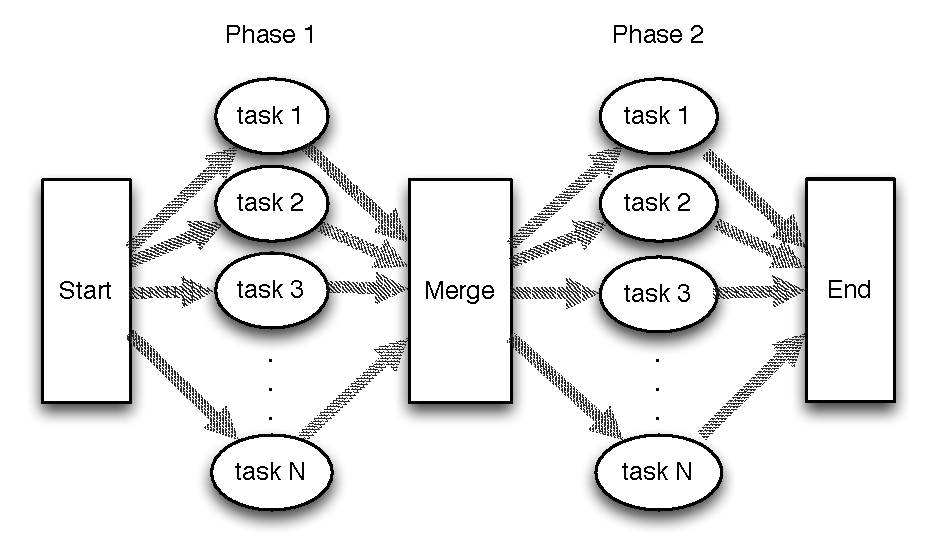
\includegraphics[width=\columnwidth]{Figures/map_reduce.pdf}
	\end{center}
	\caption{Cloud computing execution model with 2 phases.}
	\label{fig:map_reduce}
\end{figure}

Each job has a targeted response time defined
by the terms of the SLA. Further, the SLA defines the amount to be
paid for completing the job by the targeted response time as well as
the penalty to be incurred if the targeted response time is not
met. 

Each task is mapped to one compute core and executes at a rate, $\sigma$. The partition of the job among tasks is
such that each task processes a similar
workload, $W$. Consequently, baring failures, tasks are expected to
complete at about the same time. Therefore, the minimal response time
of each task, when no failure occurs, is
$t_{min}~=~\frac{W}{\sigma_{max}}$, where $\sigma_{max}$ is the maximum execution rate. This is also the minimal response
time of the entire phase. 


\subsection{Optimization}
This part describes an optimization problem for a single job on top of the Cloud computing execution model described above. Using this
framework we compute profit-optimized execution rates for Shadow Replication with dual modular redundancy (i.e., one shadow process per main process): 

\begin{equation}
\label{optimization_problem}
%\setlength{\abovedisplayskip}{14pt}
\begin{alignedat}{2}
\max_{\sigma_m,\sigma_b,\sigma_a}     & E[profit] \\
s.t.                                 & 0 \leq \sigma_m \leq \sigma_{max} \\
                                     & 0 \leq \sigma_b \leq \sigma_{m} \\
                                     & 0 \leq \sigma_a \leq \sigma_{max} 
\end{alignedat}
\end{equation}
We assume that processor execution 
rates are continuous and use nonlinear optimization techniques
to solve the above optimization problem. 

In order to earn profit, service providers must either increase
income or decrease expenditure. We take both factors into
consideration for the purpose of maximizing profit while meeting
customer's expectation. In our model, the expected profit is defined as the expected reward minus the expected expense.

\begin{equation}
E[\text{profit}]=E[\text{reward}]-E[\text{expense}]
\end{equation}

\subsubsection{Reward Model}
\label{sec:sla_reward_model}

The Cloud SLA terms and conditions can be diverse and
complex. To focus on the performance and reliability
aspects of the SLA, we define the reward model based on job completion
time. Platform as a Service (PaaS) companies will continue to become
more popular, causing an increase in SLAs using job completion time as
their performance metric. We are already seeing this appear in
web-based remote procedure calls and data analytic requests.

As depicted in Figure \ref{fig:reward}, customers expect that their
job deployed on Cloud finishes by a mean response time $t_{R_1}$.  As a
return, the service provider earns a certain amount of reward, denoted by R,
for satisfying customer's requirements. However, if the job cannot be
completed by the expected response time, the provider loses a fraction of $R$
proportional to the delay incurred. For large delay, the profit loss may translate into a penalty that the CSP must pay to the customer. In this model, the maximum penalty $P$ is paid if the
delay reaches or exceeds $t_{R_2}$. The four
parameters, $R$, $P$, $t_{R_1}$ and
$t_{R_2}$, completely define the reward model. 
It would be trivial to extend this reward model to any convex function, but we will not bother to do so.

\begin{figure}[t]	
	\begin{center}
		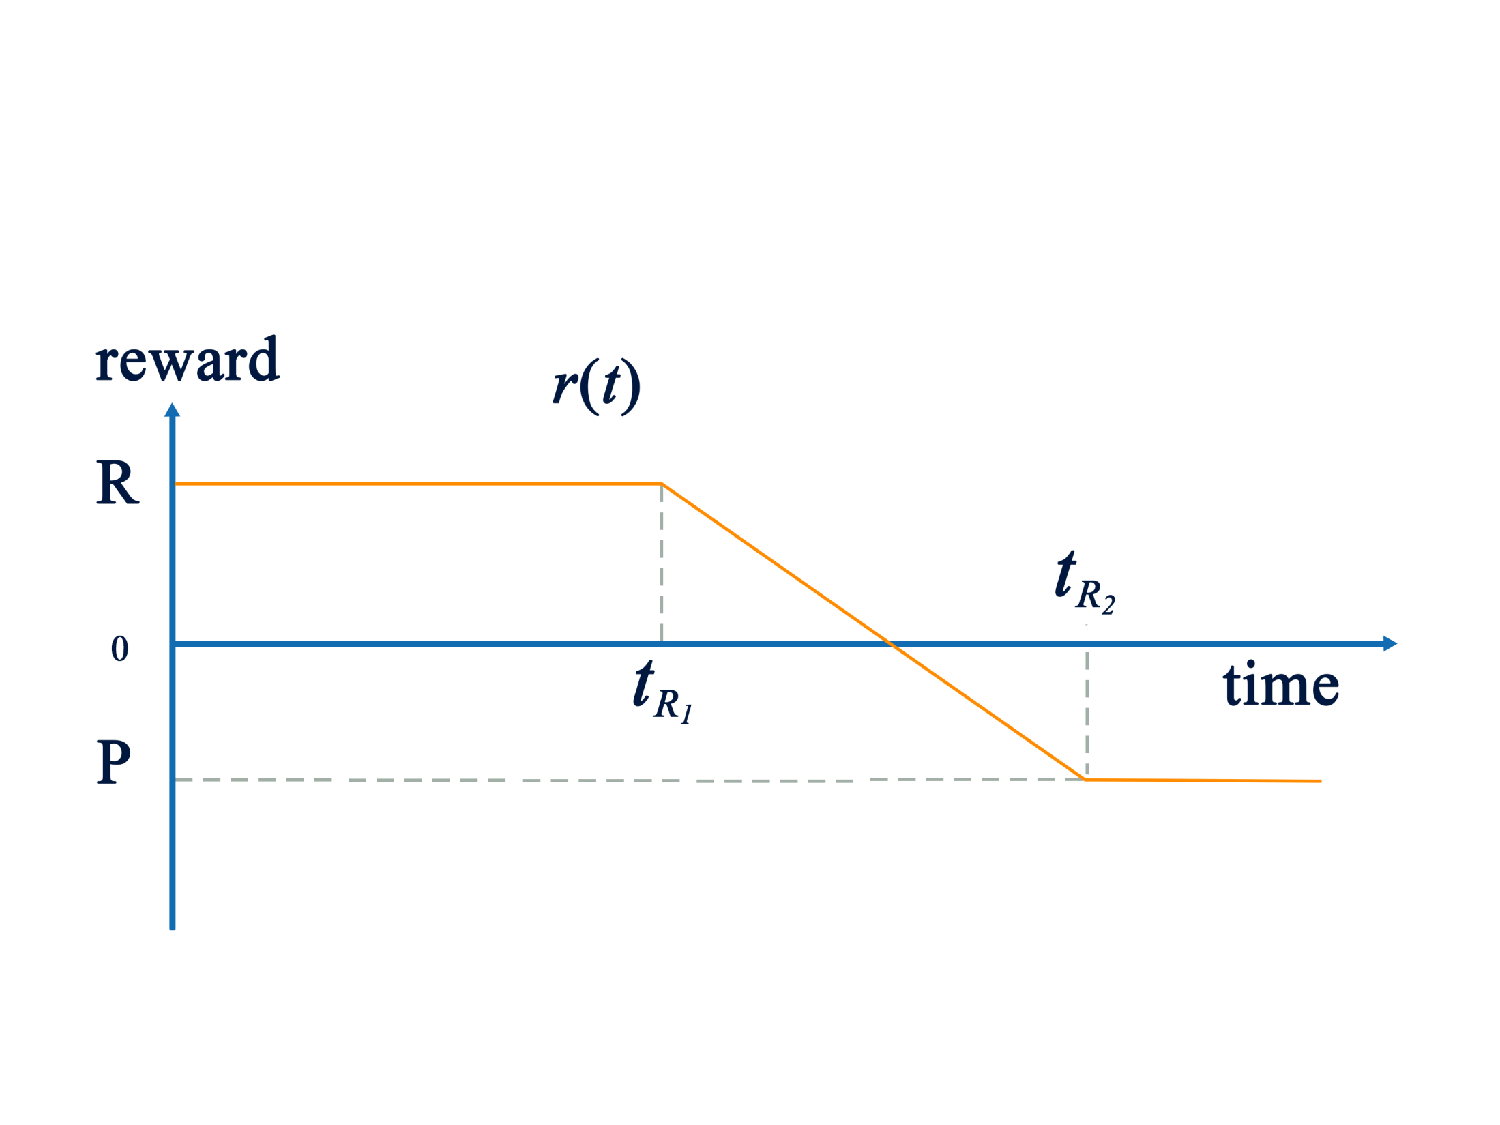
\includegraphics[width=0.8\columnwidth]{Figures/reward.pdf}
	\end{center}
	\caption{A reward model for Cloud computing.}
	\label{fig:reward}
\end{figure}


When applying Shadow Replication with dual modular redundancy to deal with crash failures, 
there are two facts that the service provider must take into account
when negotiating the terms of the SLA. The first is the response time
of the main process assuming no failure (Figure
\ref{fig:sc_no_fail} and Figure \ref{fig:sc_shadow_fail}). This
results in the following completion time:
\begin{equation}
t_c^m=W/\sigma_m
\label{eq:tcm}
\end{equation}

If the main process fails (shown in Figure \ref{fig:sc_main_fail}), the
task completion time by shadow process is the time of the failure,
$t_f$, plus the time necessary to complete the remaining work.

\begin{equation}
t_c^s=t_f+\frac{W-t_f \times \sigma_b}{\sigma_a}
\label{eq:tcs}
\end{equation}

\subsubsection{Failure Model}
Failure can occur at any point during the execution of the main or
shadow process. Our assumption is that at most one failure occurs,
therefore if the main process fails it is implied that the shadow will
complete the task without failure. We can make this assumption because
we know the failure of any one node is rare, thus the failure
of any two specific nodes is very unlikely.

We assume that two probability density functions, $f_m(t_f)$ and
$f_s(t_f)$, exist which express the probabilities of the main and shadow
process failing at time $t_f$, separately. The model does not assume a
specific distribution. However, in the remainder of this section we use
an exponential probability density function, $f_m(t_f)=f_s(t_f)=\lambda
e^{-\lambda t_f}$, of which the mean time between failures (MTBF) is $\frac{1}{\lambda}$.

\subsubsection{Power and Energy Models}
This work assumes DVFS as the underlying execution rate control mechanism. 
DVFS has been widely exploited as a technique to reduce CPU dynamic power~\cite{pillai2001real,flautner2001automatic}. It
is well known that one can reduce the dynamic CPU power consumption at
least quadratically by reducing the execution rate linearly. The
dynamic CPU power consumption of a computing node executing at rate
$\sigma$ is given by the function $p_d(\sigma)=\sigma^n$ where $n \ge 2$.


In addition to the dynamic power, CPU leakage and other components
(memory, disk, network etc.) all contribute to static power
consumption, which is independent of the CPU rate. In this thesis we
define static power as a fixed fraction of the node power consumed
when executing at maximum rate, referred to as $\rho$. Hence, node power consumption is expressed as
$p(\sigma)=\rho \times \sigma_{max}^n + (1-\rho)\times \sigma^n$. When the execution rate is zero
the machine is in a sleep state, powered off or not assigned as a
resource; therefore it will not be consuming any power, static or
dynamic.  Throughout this thesis we assume that dynamic power is cubic
in relation to
rate~\cite{rusu2003maximizing,zhai2004theoretical}, therefore the
overall system power when executing at rate $\sigma$ is defined as:
\begin{equation}
p(\sigma) = \begin{cases} \rho \sigma_{max}^3 + (1-\rho) \sigma^3 & \mbox{if } \sigma > 0 \\ 
                          0 & \mbox{if } \sigma = 0 \end{cases}
\label{eq:power_model}
\end{equation}

Using the power model given by Equation~\ref{eq:power_model}, the
energy consumed by a process executing at rate $\sigma$ during an
interval $T$ is given by
\begin{equation}
E(\sigma,T) = p(\sigma) \times T
\end{equation}


Corresponding to Figure~\ref{fig:sc_overview}, there are three cases to consider: main and shadow both succeed, shadow fails, 
and main fails. As described earlier, the case of both the main and
shadow failing is very rare and will be ignored. The expected
energy consumption for a single task is then the weighted average of
the energy consumption in the three cases.

First consider the case where no failure occurs and the main process
successfully completes the task at time $t_c^m$, corresponding to Figure~\ref{fig:sc_no_fail}.
\begin{equation}
E_1 =  ( 1-\int_0^{t_c^m}f_m(t)dt) \times (1 - \int_0^{t_c^m} f_s(t)dt) \times (  E(\sigma_m,t_c^m) + E(\sigma_b,t_c^m))
\label{eq:energy_no_failure}
\end{equation}
The product of the first two factors is the probability of fault-free execution of the main
process and shadow process. Then we multiple this probability by the
energy consumed by the main and the shadow process during this fault
free execution, ending at $t_c^m$.

Next, consider the case where the shadow process fails at some point
before the main process successfully completes the task, corresponding to Figure~\ref{fig:sc_shadow_fail}.
\begin{equation}
E_2 = (1-\int_0^{t_c^m}f_m(t)dt) \times 
      \int_0^{t_c^m}(E(\sigma_m,t_c^m)+E(\sigma_b,t)) \times f_s(t)dt
\label{eq:energy_shadow_fail}
\end{equation}
The first factor is the probability that the main process does not
fail, and the probability of shadow fails is included in the second factor which also contains the energy consumption since it depends on the shadow failure time. Energy consumption comes from the main process until the completion of the task,
and the shadow process before its failure.

The one remaining case to consider is when the main process fails and
the shadow process must continue to process until the task completes,
corresponding to Figure \ref{fig:sc_main_fail}.
\begin{equation}
E_3 = (1-\int_0^{t_c^m}f_s(t)dt) \times \int_0^{t_c^m}(E(\sigma_m,t)+ E(\sigma_b,t)+E(\sigma_a,t_c^s-t))f_m(t)dt
\label{eq:energy_main_fail}
\end{equation}
Similarly, the first factor expresses the probability that the shadow process does
not fail. In this case, the shadow process executes from the beginning to
$t_c^s$ when it completes the task. However, under our ``at most one
failure'' assumption, the period during which shadow process may fail
ends at $t_c^m$, since the only reason why shadow process is still in
execution after $t_c^m$ is that main process has already failed. There
are three parts of energy consumption, including that of main process
before main's failure, that of shadow process before main's failure,
and that of shadow process after main's failure, all of which depend
on the failure occurrence time. 

The three equations above describe the expected energy consumption by a
pair of main and shadow processes for completing a task under
different situations. However, under our system model it might be the
case that those processes that finish early will wait idly and
consume static power if failure delays one task. If it is the case
that processes must wait for all tasks to complete, then this energy
needs to be accounted for in our model. The probability of this is the probability that at least one main process fails,
referred to as the system level failure probability.
\begin{equation}
P_f=1-(1-\int_0^{t_c^m}f_m(t)dt)^N
\label{eq:prob_of_one_main_failure}
\end{equation}
Hence, we have the fourth equation corresponding to the energy consumed  by some processes while waiting in idle. 
\begin{equation}
  \begin{split}
  E_4 = & ( 1-\int_0^{t_c^m}f_m(t)dt) \times (1 - \int_0^{t_c^m} f_s(t)dt) \times  P_f \times 2E(0,t_c^j-t_c^m)  \\ & + \int_0^{t_c^m}f_s(t)dt \times  (1-\int_0^{t_c^m}f_m(t)dt) \times P_f \times E(0,t_c^j-t_c^m) 
  \end{split}
\end{equation}
Corresponding to the first case, neither main process nor shadow
process fails, but both of them have to wait in idle from task
completion time $t_c^m$ to the last task's completion (by a shadow
process) with probability $P_f$. Under the second case, only the main
process has to wait if some other task is delayed since its shadow
process has already failed. These two aspects are accounted in the
first and second lines in $E_4$ separately.  We use the expected
shadow completion time $t_c^j$ as an approximation of the latest task
completion time which is also the job completion time.


By summing these four parts and then multiplying it by $N$ we will have
the expected energy consumed by Shadow Replication for completing a
job of $N$ tasks.
\begin{equation}
E[\text{energy}]=N \times (E_1 + E_2 + E_3 + E_4)
\label{eq:total_energy}
\end{equation}

\subsubsection{Reward and Expense}
Reward is the amount paid by customer for the cloud computing
services that they utilize. It depends on the reward function $r(t)$,
depicted in Figure~\ref{fig:reward}, and the actual job completion
time. Therefore, the income should be either $r(t_c^m)$, if all main
processes can complete without failure, or $r^*(t_c^s)$ otherwise. It
is worth noting that the reward in case of failure should be
calculated based on the last completed task, which we approximate by
calculating the expected time of completion allowing us to derive the
expected reward, i.e. $r^*(t_c^s)=\frac{\int_0^{t_c^m}r(t_c^s) \times
f_m(t)dt}{\int_0^{t_c^m}f_m(t)dt}$. Therefore, the expected reward is approximated by the following equation.
\begin{equation}
E[\text{reward}]= (1-P_f) \times r(t_c^m) + P_f \times r^*(t_c^s)
\end{equation}

%% there is some hand-waving maddness above, unclear how to fix? -bnm

The first part is the reward earned by the main process times the
probability that all main processes would complete tasks without
failure. If at least one main process fails, that task would have to
be completed by a shadow process. As a result, the second part is the
reward earned by shadow process times the system level failure probability.

If $C$ is the charge expressed as dollars per unit of energy consumption
(e.g. kilowatt hour), then the expected expenditure would be $C$ times
the expected energy consumption for all $N$ tasks:
\begin{equation}
E[\text{expense}] = C \times E[\text{energy}]
\label{eq:expense}
\end{equation}

However, the expenditure of running the cloud computing service is more
than just energy, and must include hardware, maintenance, and human
labor. These costs can be accounted for by amortizing these costs into the
static power factor, $\rho$. Because previous studies have
suggested
that energy will become a dominant factor~\cite{elnozahy2003energy,raghavendra2008no}, we decided to focus on this
challenge and leave other aspects to future work.

\begin{table}[!h]
\caption{Symbols used in reward-based optimal Shadow Replication.}
\centering
\begin{tabular}{|r | c |}
\hline 
Symbols                          & Definition                         \\
\hline \hline
$W$                               & Task workload                    \\
\hline
$N$                               & Number of tasks                 \\
\hline
$r(t)$                          & Reward function       \\
\hline
$R$, $P$                            & Maximum reward and penalty      \\
\hline
$t_{R_1}$, $t_{R_2}$             & Response time thresholds  \\
\hline
$C$                               & Unit price of energy            \\
\hline
$\rho$                          & Static power ratio                 \\
\hline
$t_c^m$, $t_c^s$, $t_c^{j}$                 & Completion time of main, shadow, and the whole job \\
\hline
$f_m()$, $f_s()$                    & Failure density function of main and shadow  \\
\hline
$\lambda$                           & Failure rate    \\
\hline
$P_f$                               & System level failure probability \\
\hline
$\sigma_m$, $\sigma_b$, $ \sigma_a$  & rates of main, shadow before and after failure \\
\hline
\end{tabular}

\label{tbl:symbols}
\end{table}

Based on the above formulation of the optimization problem, the
MATLAB Optimization Toolbox was used to solve the
resulting nonlinear optimization problem. The parameters of this
problem are listed in Table~\ref{tbl:symbols}. 


\section{Profit-aware Stretched Replication}
We compare Shadow Replication to two other replication techniques,
traditional replication and profit-aware stretched replication.
Traditional replication requires that the two processes always execute
at the same rate $\sigma_{max}$. Unlike traditional replication,
Shadow Replication is dependent upon failure detection, enabling the
replica to increase its execution rate upon failure and maintain the
targeted response time, thus maximizing profit. While this is the case
in many computing environments, there are cases where failure
detection may not be possible. To address this limitation, we propose
profit-aware stretched replication, whereby both the main process and
the shadow execute independently at stretched rates to meet the
expected response time, without the need for failure
detection. In profit-aware stretched replication, both the main and
shadow execute at rate $\sigma_r$, derived by optimizing the profit
model.  For both traditional replication and stretched replication,
the task completion time is independent of failure and can be directly
calculated as:
\begin{equation}
t_c=\frac{W}{\sigma_{max}} \text{ or } t_c=\frac{W}{\sigma_r}
\end{equation}

Since all tasks will have the same completion time, the job completion
time would also be $t_c$. Further, the expected income, which depends
on negotiated reward function and job completion time, is independent
of failure:
\begin{equation}
E[reward]=r(t_c)
\end{equation}

Since both traditional replication and profit-aware stretched
replication are special cases of our Shadow Replication paradigm where
$\sigma_m=\sigma_b=\sigma_a=\sigma_{max}$ or
$\sigma_m=\sigma_b=\sigma_a=\sigma_r$ respectively, we can easily derive the
expected energy consumption using Equation~\ref{eq:total_energy} with $E_4$
fixed at 0 and then compute the expected expense using Equation~\ref{eq:expense}.

\section{Re-execution} 
Contrary to replication, re-execution initially assigns a single
process for the execution of a task. If the original task fails, the
process is re-executed. In the Cloud computing execution framework,
this is equivalent to a checkpoint/restart, in which the checkpoint is
implicitly taken at the end of each phase, and because the tasks are
loosely coupled they can restart independently. 

Based on the one failure assumption, two cases must be considered to
calculate the task completion time. If no failure occurs, the task
completion time is:
\begin{equation}
t_c=\frac{W}{\sigma_{max}}
\end{equation}
In case of failure, however, the completion time is equal to the sum
of the time elapsed until failure and the time needed for
re-execution. Again, we use the expected value
$t_f^*=\frac{\int_0^{t_c}t \times f_m(t)dt}{\int_0^{t_c}f_m(t)dt}$ to
approximate the time that successfully completed processes have to
spend waiting for the last one.

Similar to Shadow Replication, the reward for re-execution is the
weighted average of the two cases:
\begin{equation}
E[\text{reward}]=(1-P_f) \times r(t_c) + P_f \times r(t_c+t_f^{*})
\end{equation}

For one task, if no failure occurs then the expected energy can be
calculated as
\begin{equation}
E_5=(1 - \int_0^{t_c} f_m(t)dt) \times (E(\sigma_{max},t_c)+ P_f \times E(0,t_f^{*}))
\label{eq:energy_first_task}
\end{equation}
If failure occurs, however, the expected energy consumption can be calculated as
\begin{equation}
E_6=\int_0^{t_c}(E(\sigma_{max},t) + E(\sigma_{max},t_c)) \times f_m(t) dt
\label{eq:energy_rexecution_task}
\end{equation}
Therefore, the expected energy by re-execution for
completing a job of $N$ tasks is
\begin{equation}
E[energy]=N \times (E_5 + E_6)
\end{equation}

\section{Evaluation}
\noindent This section evaluates the expected profit of each of the fault tolerance
methods discussed above under different system environments. We have identified 5
important parameters which affect the expected profit:
\begin{itemize}
\item Static power ratio $\rho$, which determines the portion of power that is unaffected by the execution rate.
\item SLA - The amount of reward, penalty and the required response times.
\item $N$ - The total number of tasks.
\item MTBF - The reliability of an individual node.
\item Workload - The size, $W$, of each individual task.
\end{itemize}



Without loss of generality, we normalize $\sigma_{max}$ to be 1, so
that all the rates can be expressed as a fraction of maximum
rate. Accordingly, the task workload $W$ is also adjusted such that
it is equal to the amount of time (in hours) required for a single
task, preserving the ratios expressed in
Figure~\ref{eq:tcm} and \ref{eq:tcs}. The price of
energy $C$ is assumed to be 1 unit. We assume that $R$ in our reward model
is linearly proportional to the number of tasks $N$ and the maximum
reward for one task is 3 units, so the total reward for a job is $3
\times N$ units.  However, for the analysis we look
at the average of expenditure and income on each task by dividing the
total expenditure and income by $N$. In our basic configuration we
assume that the static power ratio is 0.5, the task size is 1 hour, the node MTBF 5 is
years, the number of tasks is $100000$, and the response time thresholds for
maximum and minimum rewards are 1.3 hours and 2.6 hours
respectively. Since the maximum power consumption is 1 unit, the
energy needed for the task with one process at maximum rate is also 1
unit. 

\subsection{Sensitivity to Static Power}

With various architectures and organizations, servers deployed at
different data centers will have different characteristics in terms of
power consumption. The static power ratio is used to abstract the
amount of static power consumed versus dynamic power.  

\begin{table}[!h]\small
	\caption{Optimal execution rates for different static power ratio. MTBF=5 years, N=100000, W=1 hour, $t_{R_1}$=1.3 hours, $t_{R_2}$=2.6 hours.}
	\centering
		\begin{tabular}{|p{1cm}|p{1cm}|p{1cm}|p{1cm}|}
		\hline
		$\rho$ & $\sigma_m$ & $\sigma_b$ & $\sigma_a$ \\
		\hline
		0.0 &	0.77 & 	0.65 & 	1.00 \\
		\hline 
		0.1 &	0.78 &	0.66 &	1.00 \\
		\hline
		0.2 &	0.83 &	0.66 &	1.00 \\
		\hline
		0.3	&   0.84 &	0.68 &	1.00 \\
		\hline
		0.4	&   0.85 &	0.70 &	1.00 \\
		\hline
		0.5	&   0.86 &	0.72 &	1.00 \\
		\hline
		0.6	&   0.87 &	0.73 &	1.00 \\
		\hline
		0.7	&	0.91 &	0.81 &	1.00 \\
		\hline
		0.8	& 	1.00 &	1.00 &	1.00 \\
		\hline
		0.9	&	1.00 &	1.00 &	1.00 \\
		\hline
		1.0	&	1.00 &	1.00 &	1.00 \\
		\hline
		\end{tabular}
	\label{tbl:rho}
\end{table}

\begin{figure}[!h]	
	\begin{center}
		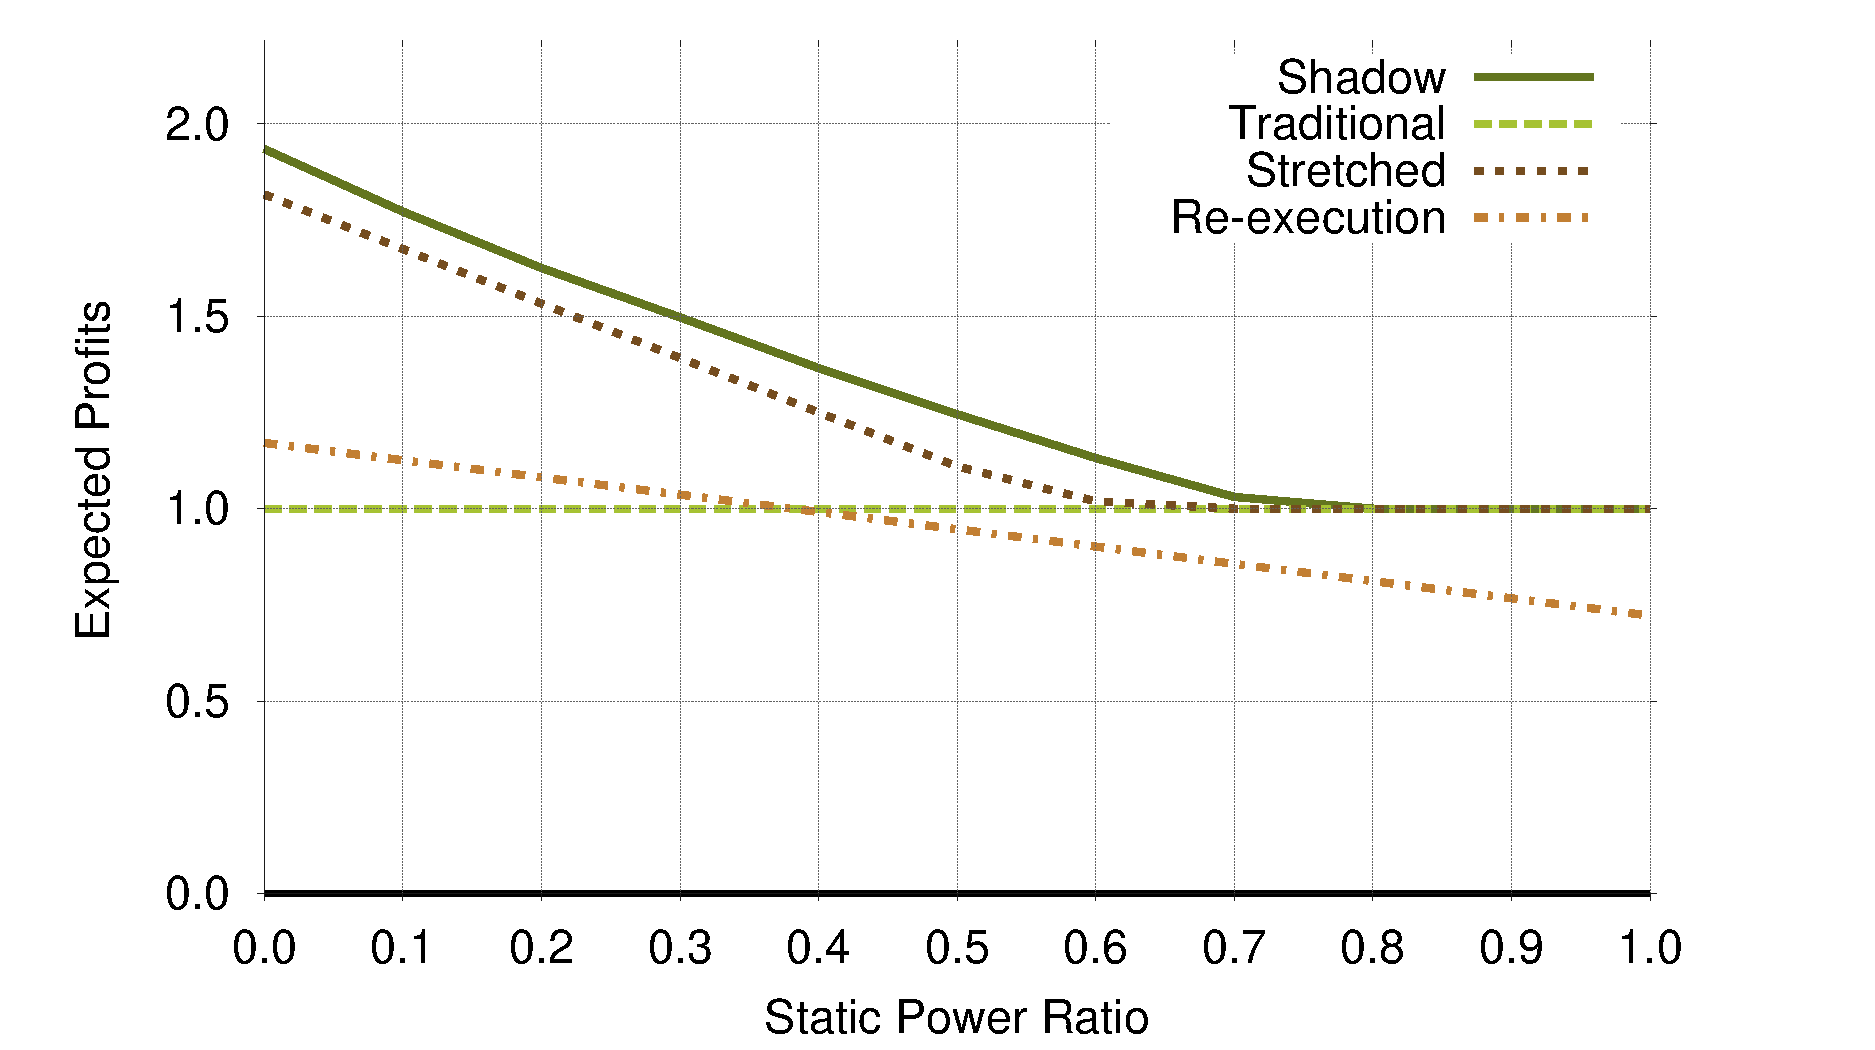
\includegraphics[width=\columnwidth]{Figures/rho_profit}
	\end{center}
	\caption{Profit for different static power ratio. MTBF=5 years, N=100000, W=1 hour, $t_{R_1}$=1.3 hours, $t_{R_2}$=2.6 hours.}
	\label{fig:rho}
\end{figure}

Table \ref{tbl:rho} shows how the profit-optimized execution rates
of Shadow Replication will change as static power increases. The execution rates increase to reduce the execution time as static power ratio increases. Observe
that $\sigma_a$ is always equal to $\sigma_{max}$, which means that after
sensing the failure of the main process, the shadow process should always
shift to maximum rate. This is expected because the optimization will
reduce the amount of work done by the shadow process before failure,
resulting in the maximum execution rate after failure, thus
minimizing the amount of repeated work. 

The potential profit gains achievable by using profit-aware
replication techniques decreases as static power increases, as is shown
in Figure~\ref{fig:rho}. The reason is that our profit-aware
techniques rely upon the fact that one can reduce energy costs by
adjusting the execution rates. Modern systems have a static power between 40\%-70\%~\cite{butts2000static}, and
it is reasonable to suspect that this will continue to be the case in the near future. Within
this target range, Shadow Replication can achieve, on
average, 19.3\% more profit than traditional replication, 8.9\% more
than profit-aware stretched replication, and 28.8\% more than re-execution.


\subsection{Sensitivity to Response Time}

Response time is critical in the negotiation of SLA as customers
always expect their tasks to complete as soon as possible. In this
section we show a sensitivity study with respect to task response
time. We vary the first threshold $t_{R_1}$ from the minimum response
time $t_{min}$ to $1.9t_{min}$, and set the second threshold $t_{R_2}$
to be always $2t_{R_1}$. We do not show results for varying the reward
and penalty values of the SLA. The reason is that changing these
values have no effect on the choice of fault tolerance methods because
they are all affected in a similar way.

\begin{table}[!h]\small
	\caption{Optimal execution rates for different response time threshold. $\rho$=0.5, MTBF=5 years, N=100000, W=1 hour.}
	\centering
		\begin{tabular}{|p{1cm}|  p{1cm}|p{1cm}|p{1cm}|}
		\hline
		$t_{R_1}$ & $\sigma_m$ & $\sigma_b$ & $\sigma_a$ \\
		\hline
		1.0	&	1.00 & 	1.00 &	1.00 \\
		\hline
		1.1	&	0.94 &	0.88 &	1.00 \\
		\hline
		1.2	&	0.89 &	0.79 &	1.00 \\
		\hline
		1.3	&	0.86 &	0.72 &	1.00 \\
		\hline
		1.4	&	1.00 &	0.00 &	1.00 \\
		\hline
		1.5	&	1.00 &	0.00 &	1.00 \\
		\hline
		1.6	&	0.84 &	0.00 &	1.00 \\
		\hline
		1.7	&	0.74 &	0.00 &	1.00 \\
		\hline
		1.8	&	0.64 &	0.00 &	1.00 \\
		\hline
		1.9	&	0.64 &	0.00 &	1.00 \\
		\hline
		\end{tabular}
	\label{tbl:t}
\end{table}

\begin{figure}[!h]	
	\begin{center}
		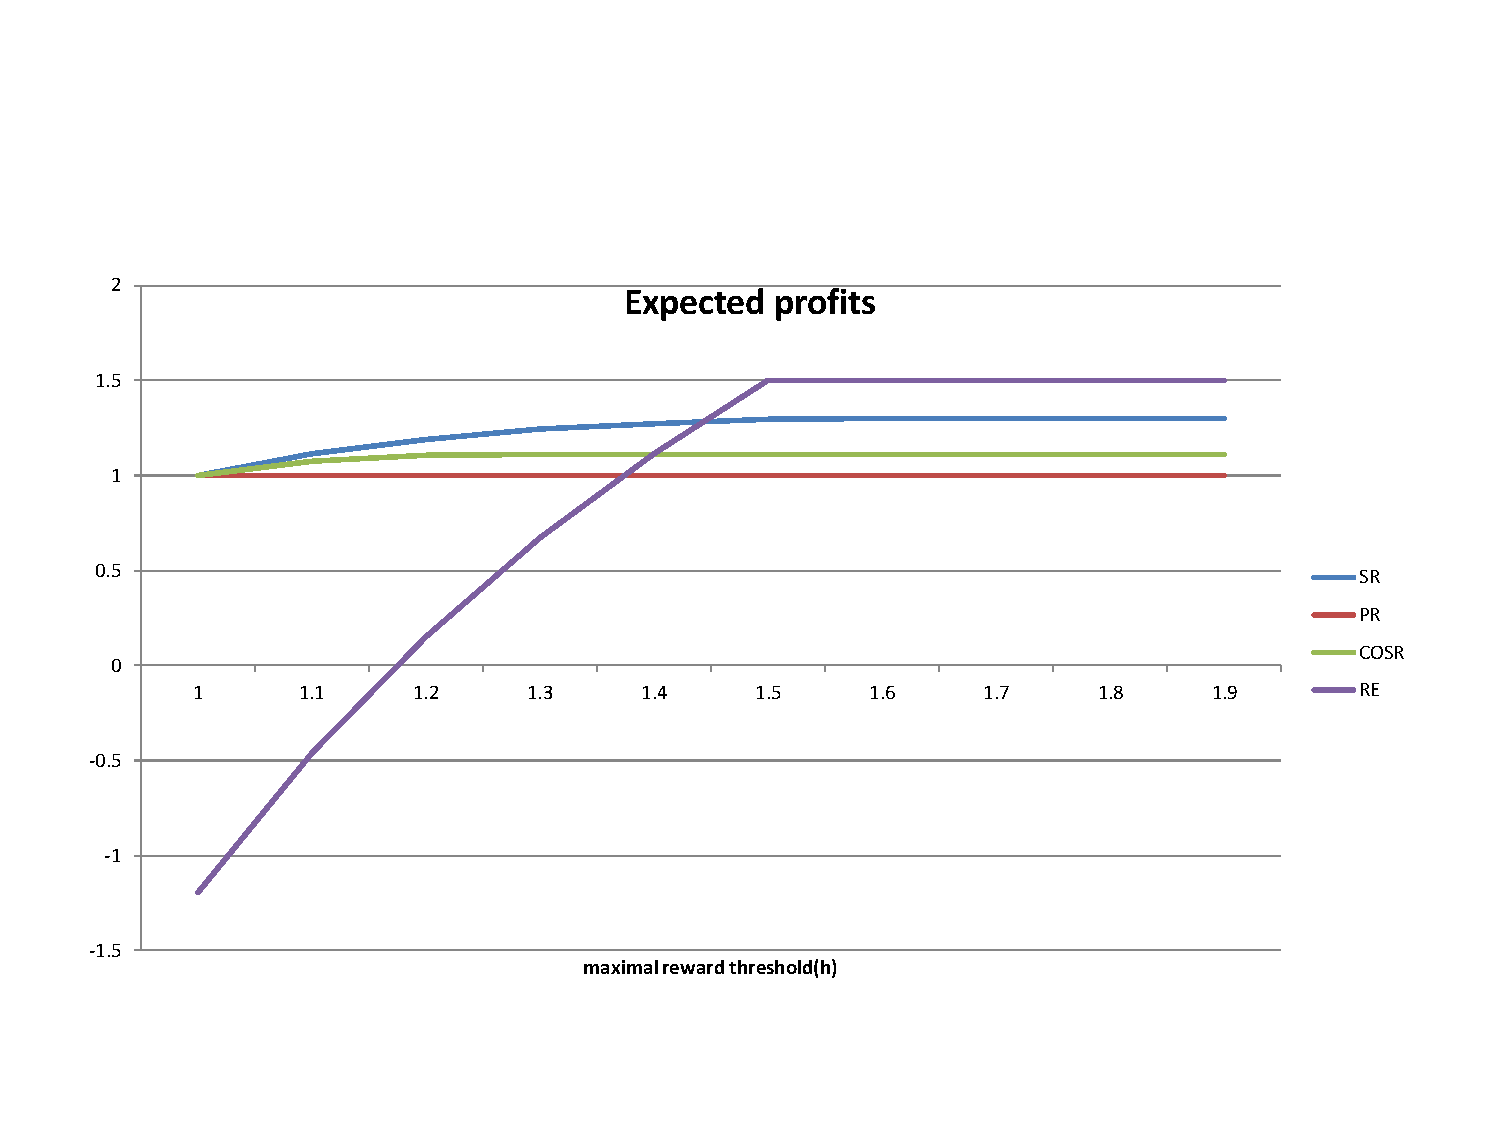
\includegraphics[width=\columnwidth]{Figures/t_profit}
	\end{center}
	\caption{Profit for different response time threshold. $\rho$=0.5, MTBF=5 years, N=100000, W=1 hour.}
	\label{fig:t}
\end{figure}

In Table~\ref{tbl:t} we see that Shadow Replication adapts the execution
rates to take advantage of the available laxity, reducing its rates
as laxity increases. It is clear that Shadow Replication has two different execution strategies separated by $t_{R_1}=1.4$: when time is critical, it uses both a main and a shadow from the very beginning to guarantee that task can be completed on time; when time is not critical, it mimics re-execution and starts its shadow only after a failure.
Also note that as $t_{R_1}$
approaches $t_{min}$, the rates of the main process and the shadow process
converge, effectively causing Shadow Replication to mimic traditional
replication when faced with time-critical jobs.

Figure~\ref{fig:t} shows the effect that targeted response time has upon
the profitability of each fault tolerance method. Compared to traditional replication, all the other methods increase their profit as the targeted
response time increases, this is expected because each of the other
techniques can make use of increased laxity in time to increase
profit. Re-execution is the most sensitive to the target response
time since it fully relies upon time redundancy, showing that it should only be used when the targeted response time is \emph{not} stringent. 
Again, Shadow Replication always achieves more profit than traditional
replication and profit-aware stretched replication, and the profit
gains are 52.8\% and 39.0\% on average. 


\subsection{Sensitivity to Number of Tasks}
The number of tasks has a direct influence upon the system level
failure probability because as the number of tasks increase the
probability that failure will occur to at least one task
increases. Recall that even one failure can hurt the total reward
significantly, and keep the other processes waiting. Thus, Shadow
Replication will adjust its execution rates to reduce the waiting
time.

\begin{table}[!h]\small
	\caption{Optimal execution rates for different number of tasks. $\rho$=0.5, MTBF=5 years, W=1 hour, $t_{R_1}$=1.3 hours, $t_{R_2}$=2.6 hours.}
	\centering
		\begin{tabular}{|r|p{1cm}|p{1cm}|p{1cm}|}
		\hline
		$N$ & $\sigma_m$ & $\sigma_b$ & $\sigma_a$ \\
		\hline
		100			&	0.80	&	0.00	&	1.00 \\
		\hline
		1,000		&	0.84	&	0.00	&	1.00 \\
		\hline
		10,000		&	1.00	&	0.00	&	1.00 \\
		\hline
		100,000		&	0.86	&	0.72	&	1.00 \\
		\hline
		1,000,000		&	0.86	&	0.72	&	1.00 \\
		\hline
		10,000,000	&	0.86	&	0.72	&   1.00 \\
		\hline
		\end{tabular}
	\label{tbl:n}
\end{table}

Table~\ref{tbl:n} is similar to Table~\ref{tbl:t} in that there are also two execution strategies. When there are few parallel tasks, shadow
replication chooses to execute the main processes at nearly full rate and keeps
the shadow processes dormant. The
reason is that it is very likely that all main processes can finish
their tasks successfully, and the need for redundancy is thus less
significant. The other case is when there is a huge number of
tasks to execute, the shadow process would keep running at a slower rate than the main to protect the main as well as save energy. Since the system level failure probability is already 0.9 when $N$ is 100000, the rates stay the same when $N \ge 100000$.

Figure \ref{fig:n} confirms that for small number of tasks
re-execution is more profitable than replication. However, re-execution is not scalable
as its profit decreases rapidly after N reaches 10000. At the same time, traditional
replication and profit-aware stretched replication are not
affected by the number of tasks because neither are affected by the
system level failure rate. On average, Shadow Replication achieves 43.5\%, 59.3\%, and 18.4\%
more profits than profit-aware stretched replication, traditional replication and re-execution, respectively. 

\begin{figure}[!h]	
	\begin{center}
			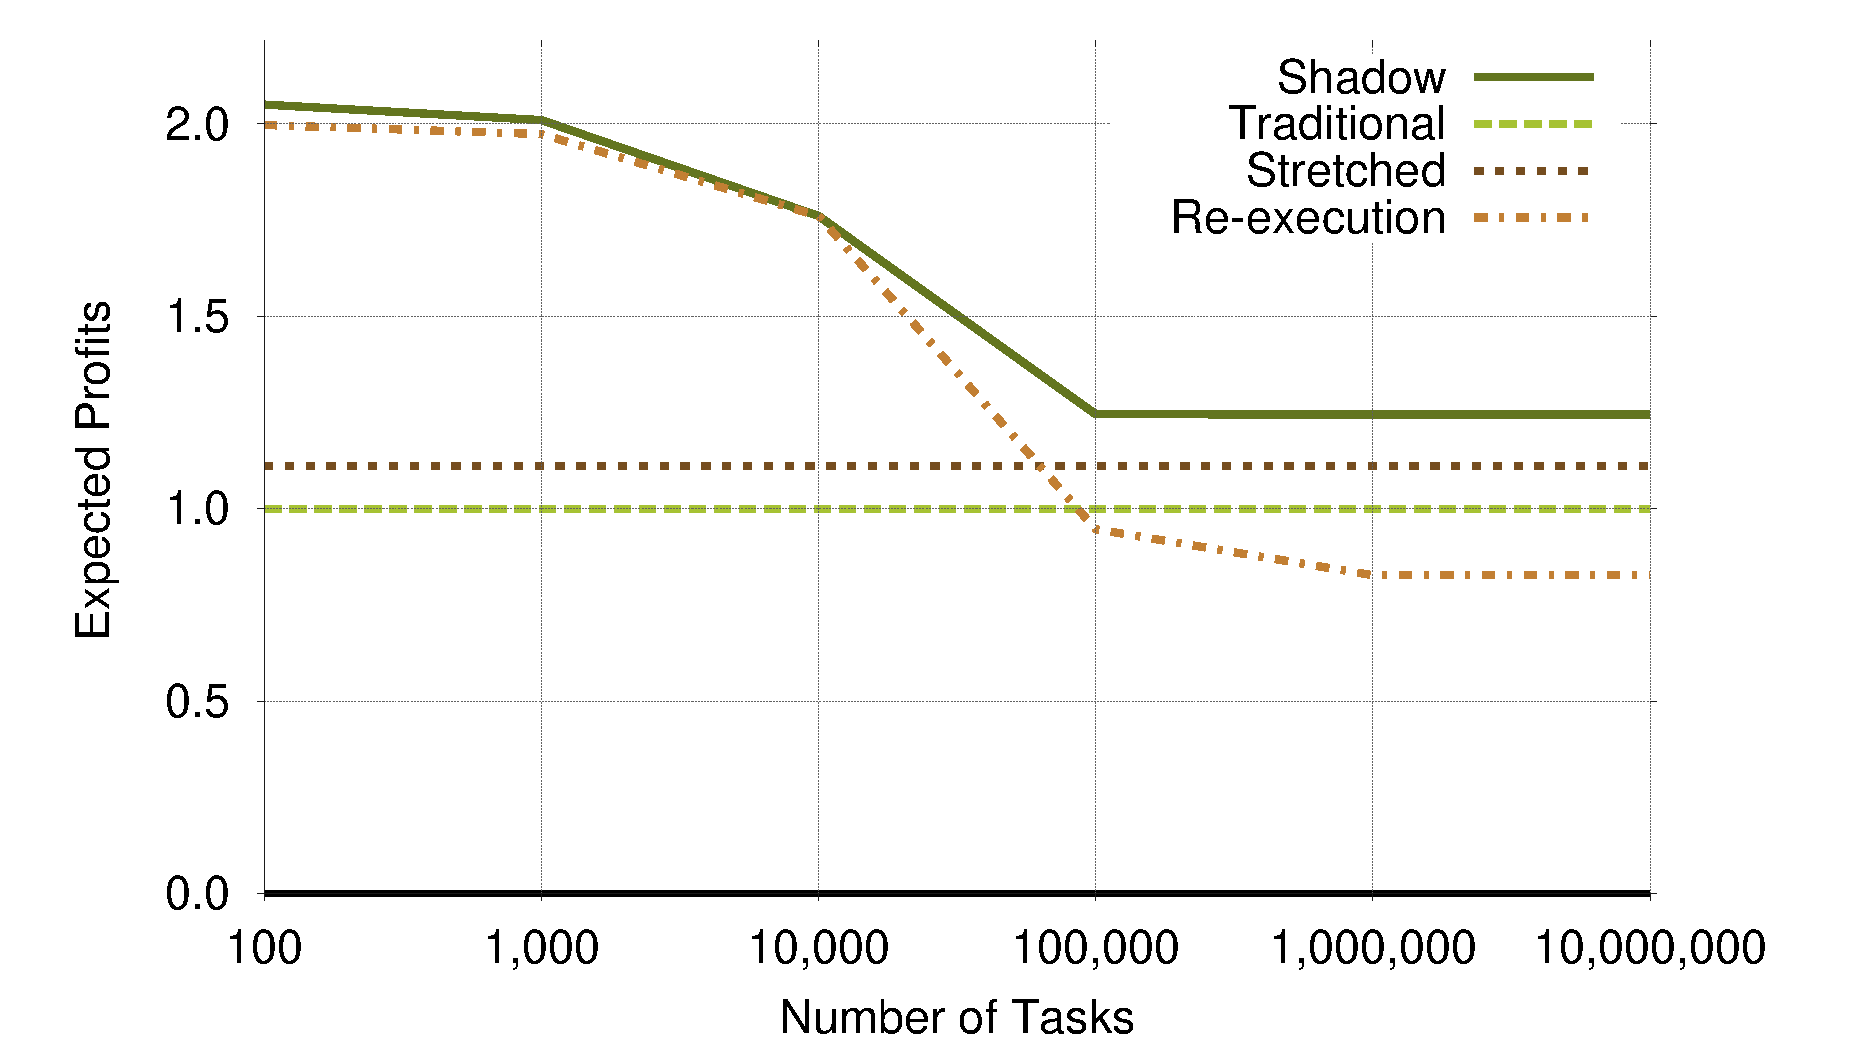
\includegraphics[width=\columnwidth]{Figures/n_profit}
	\end{center}
	\caption{Profit for different number of tasks. $\rho$=0.5, MTBF=5 years, W=1 hour, $t_{R_1}$=1.3 hours, $t_{R_2}$=2.6 hours.}
	\label{fig:n}
\end{figure}

\subsection{Sensitivity to Failure Vulnerability}

The ratio between task size and node MTBF represents the task's
vulnerability to failure. Specifically, it is an approximation of the
probability that failure occurs during the execution of the task. In our
analysis we found that increasing task size will have the same effect
as reducing node MTBF. Therefore, we analyze these together using the
\textit{vulnerability to failure}, allowing us to analyze a wider range of
system parameters.

\begin{table}[!h]\small
	\caption{Optimal execution rates for different task size over MTBF. $\rho$=0.5, N=100000, $t_{R_1}$=1.3 hours, $t_{R_2}$=2.6 hours.}
	\centering
		\begin{tabular}{|c|p{1cm}|p{1cm}|p{1cm}|}
		\hline
		$W/MTBF$ & $\sigma_m$ & $\sigma_b$ & $\sigma_a$ \\
		\hline
		2E-10	&	0.79 &	0.00 &	1.00 \\
		\hline
		2E-09	&	0.79 &	0.00 &	1.00 \\
		\hline
		2E-08	&	0.80 &	0.00 &	1.00 \\
		\hline
		2E-07	&	0.84 &	0.00 &	1.00 \\
		\hline
		2E-06	&	1.00 &	0.00 &	1.00 \\
		\hline
		2E-05	&	0.86 &	0.72 &	1.00 \\
		\hline
		2E-04	&	0.86 &	0.72 &	1.00 \\
		\hline
		2E-03	&	0.86 &	0.72 &	1.00 \\
		\hline
		%2E-02	&	0.86 &	0.72 &	1.00 \\
		%\hline
		\end{tabular}
	\label{tbl:mtbf}
\end{table}

\begin{figure}[!h]	
	\begin{center}
			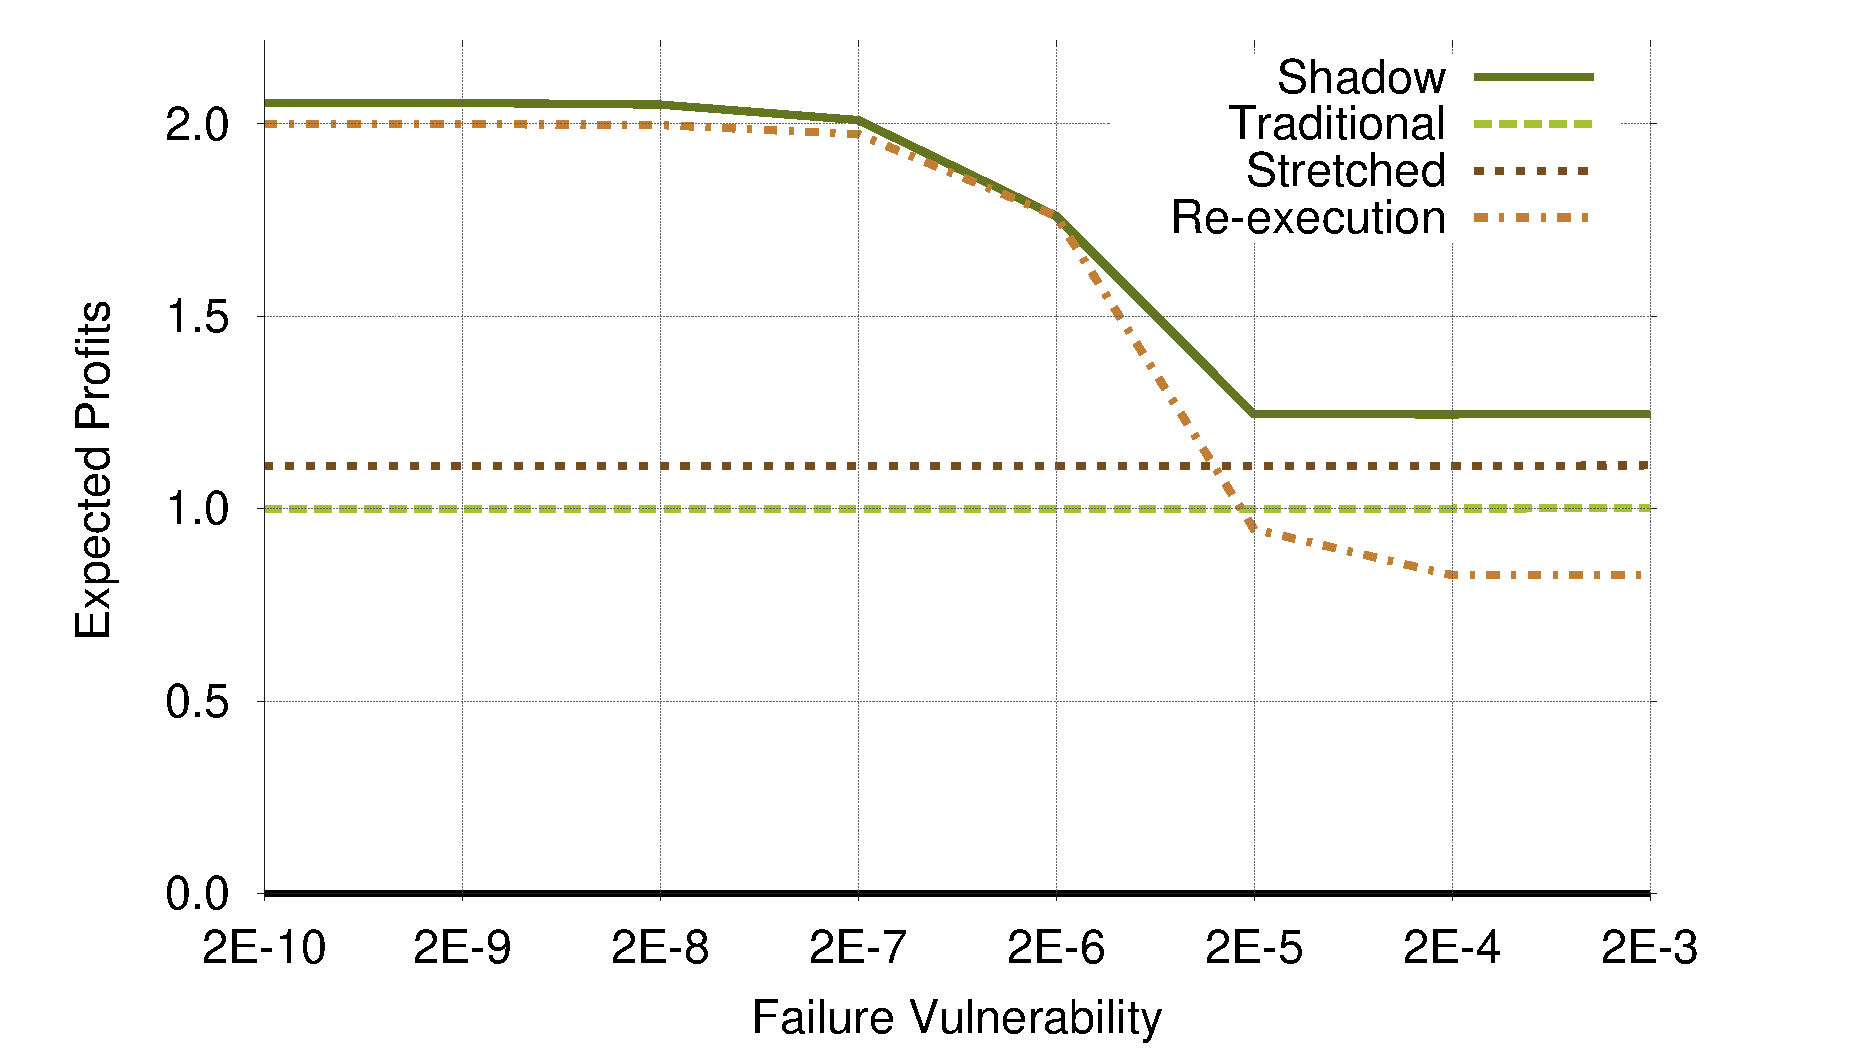
\includegraphics[width=\columnwidth]{Figures/mtbf_profit}
	\end{center}
	\caption{Profit for different task size over MTBF. $\rho$=0.5, N=100000, $t_{R_1}$=1.3 hours, $t_{R_2}$=2.6 hours.}
	\label{fig:mtbf}
\end{figure}

As seen in Table~\ref{tbl:mtbf}, when the vulnerability to
failure is low the execution rates for the shadow process is such
that no work is done before failure. However, as the
vulnerability increases, the shadow process performs more work before
failure. This is analogous to what we observed as we increased the
number of tasks (Table~\ref{tbl:n}). As expected,
re-execution is desired when the vulnerability to failure is
low. As always, Shadow Replication can adjust its execution strategy to maximize the profits, as shown in Figure~\ref{fig:mtbf}.

\subsection{Application Comparison}

To compare the potential benefit of Shadow Replication, we evaluate
the expected profit of each resilience technique using three different
benchmark applications representing a wide range of
Cloud workloads~\cite{mrbs}: Business Intelligence, Bioinformatics and
Recommendation System. The business intelligence benchmark application
is a decision support system for a wholesale supplier. It emphasizes
executing business-oriented ad-hoc queries using Apache Hive. The
bioinformatics application performs DNA sequencing, allowing genome
analysis on a wide range of organisms. The recommendation system is
similar to those typically found in e-commerce sites which, based upon
browsing habits and history, recommends similar
products.

\begin{table}[h]
	\centering
    	\caption{Cloud benchmark applications~\cite{mrbs}.}
		\begin{tabular}{|c|c|}
			\hline
			Application               & Processing Rate \\
			\hline\hline
			Business Intelligence     & 3.3 (MB/s)      \\ \hline
			Bioinformatics            & 6.6 (MB/s)      \\ \hline
			Recommendation System     & 13.2 (MB/s)     \\
			\hline
       \end{tabular}
	   \label{tbl:application_processing_rates}
\end{table}

Using the results of the experiments reported in \cite{mrbs}, we
derived the time required to process data for each application type (Table~\ref{tbl:application_processing_rates}). We assume that
these processing rates per task will not change when scaling the
applications to future cloud environments. This is a reasonable
assumption given that map-reduce tasks are loosely coupled and data
are widely distributed, therefore data and task workload will scale
linearly.

In Figure \ref{fig:app_compare} we compare the expected
profit for each application using each of the 4 resilience techniques. 
We consider two data sizes expected in future
cloud computing environments, 500TB and 2PB. The figure shows that
for business intelligence applications, Shadow Replication achieves significantly larger profits for both data sizes. This
is because business intelligence applications tend to be I/O intensive,
resulting in longer running tasks, whereas recommendation systems tend
to require little I/O, resulting in shorter running tasks, making
re-execution as good as Shadow Replication. Bioinformatics tends to be in between
these two applications, resulting in Shadow Replication performing better
when processing large datasets (2 PB) but not outstanding on smaller
datasets (500 TB). The take-away from this evaluation is that for the
shown system parameters, if phase execution is short, then re-execution
performs as well as Shadow Replication. Alternatively, if a phase is long (20 minutes or
greater), then Shadow Replication can be as much as 47.9\% more
profitable than re-execution. The previous sensitivity analysis can be
used to extrapolate expected profit for different system parameters.


\begin{figure}[!h]
	
	\begin{center}
	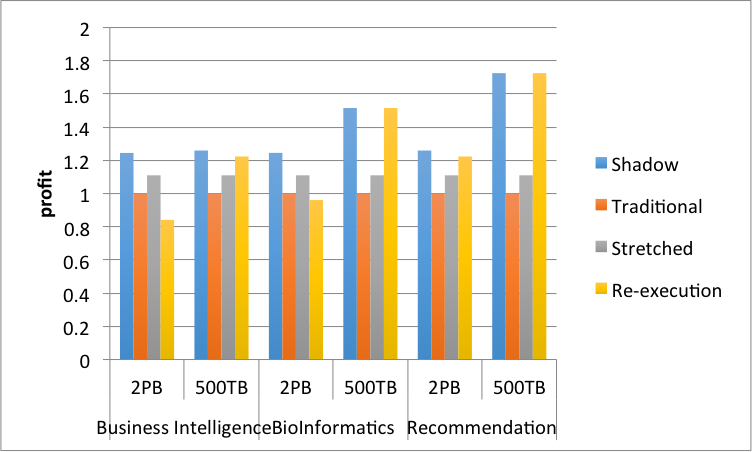
\includegraphics[width=\columnwidth]{Figures/application_comparison.png}
	\end{center}
	\caption{Application comparison. $\rho$=0.5, N=$500000$, $t_{R_1}$=$1.3t_{min}$, $t_{R_2}$=$2.6t_{min}$.}
	\label{fig:app_compare}
\end{figure}





\section{Summary}

In this work we focus on the objective of satisfying SLA in Cloud Computing and demonstrate that Shadow Replication is capable of achieving multi-dimensional QoS goals. 
To assess the performance of the Shadow Replication, an analytical framework is developed and 
an extensive performance evaluation study is carried out. 
In this study, system properties that affect the
profitability of fault tolerance methods, namely failure rate,
targeted response time and static power, are identified. The failure rate is
affected by the number of tasks and vulnerability of the task
to failure. The targeted response time represents the 
clients' desired job completion time.  
Our performance evaluation shows that in all cases, Shadow Replication outperforms
existing fault tolerance methods. Furthermore, Shadow
Replication will converge to traditional replication when target response time is stringent, and to re-execution when target response time is relaxed or failure is unlikely.


   






\chapter{Applying Lazy Shadowing to extreme-scale systems}
\label{chapter:scale}
Enabling Lazy Shadowing for resiliency in extreme-scale computing 
brings about a number of challenges and design decisions, including the applicability of this concept to a large number of 
tasks executing in parallel, the effective way to control shadows' execution rates, and the runtime mechanisms and 
communications support to ensure efficient coordination between a 
main and its shadow.
Taking into consideration the main characteristics of compute-intensive and highly-scalable applications, we design two novel techniques, referred to as {\it shadow collocation} and {\it shadow leaping}, 
and integrate them with Shadow Replication to form a more efficient and scalable paradigm that we call Lazy Shadowing.
%in order to achieve high-tolerance to failure while minimizing delay and energy consumption.

%We consider the class of compute-intensive and strongly-scaled applications, executing on a large-scale multi-core computing infrastructure~\cite{doe_ascr_exascale_2011}. 
%We use $W$ to denote the size of an application workload, and assume that the workload is split into a set of tasks, $T$, which execute in parallel. 
%Assuming the maximum execution rate is $\sigma_{max}=1$, the failure-free completion time of the application is $W/|T|$. 
%Given the prominence of MPI in HPC environments, we assume message passing as the communication mechanism between tasks. 
%The execution is composed of a set of iterations separated by synchronization barriers. 

\section{Shadow collocation}
To control the processes' execution rate, DVFS can be applied while each process resides on one core exclusively. 
The effectiveness of DVFS, however, may be markedly 
limited by the granularity of voltage control, the number of frequencies available, and the negative effects on 
reliability~\cite{Eyerman:2011:FDU:1952998.1952999,Keller:EECS-2015-257,chandra2008defect,zhao2008reliability}. 
An alternative is to collocate multiple processes on each core while keeping all the cores executing at maximum frequency. 
Then time sharing can be used to achieve the desired execution rates for each collocated process. 
Since this approach collocates multiple processes on each  core, it simultaneously reduces the number of compute nodes required and 
reduces the power consumption. 


%We use the term core to represent the resource allocation unit (e.g., a
%CPU core, a multi-core CPU, or a cluster node), so that our algorithm is agnostic to the
%granularity of the hardware platform~\cite{casanova_inria_2012}. Each main process executes on one core exclusively to achieve maximum throughput.  
%On the other hand, we collocate multiple shadows on a single core and use time sharing to achieve the desired execution rates.
To execute an application of $M$ tasks, $N=M+S$ cores are required, where $M$ is a multiple of $S$. Each main is allocated one core (referred to as \textit{main core}), while $\alpha=M/S$ (referred to as \textit{collocation ratio}) shadows are collocated on a core (\textit{shadow core}). 
The $N$ cores are grouped into $S$ sets, each of which we call a \textit{shadowed set}. Each shadowed set contains $\alpha$ main cores and 1 shadow core.
This is illustrated in Figure~\ref{fig:sc_mapping}.  

Collocation has an important ramification with respect to the resilience of the system. Specifically, 
one failure can be tolerated in each shadowed set. If a shadow core fails, all the shadows in the 
shadowed set will be lost without interrupting the execution of the mains. 
On the other hand, if a main core fails, the associated shadow will be promoted to a new main, and all 
the other collocated shadows will be terminated to speed up the new main.
Consequently, a failure, either in main or shadow core, will result in losing all the shadows in the shadowed set, thereby losing the tolerance to any other failures. After the first failure, a shadowed set becomes \emph{vulnerable}\footnote{Rejuvenation techniques, such as restarting the lost shadows from the state of current mains on spare cores, can be used to eliminate vulnerability.}. 
 
\begin{figure}[!b]
  \begin{center}
    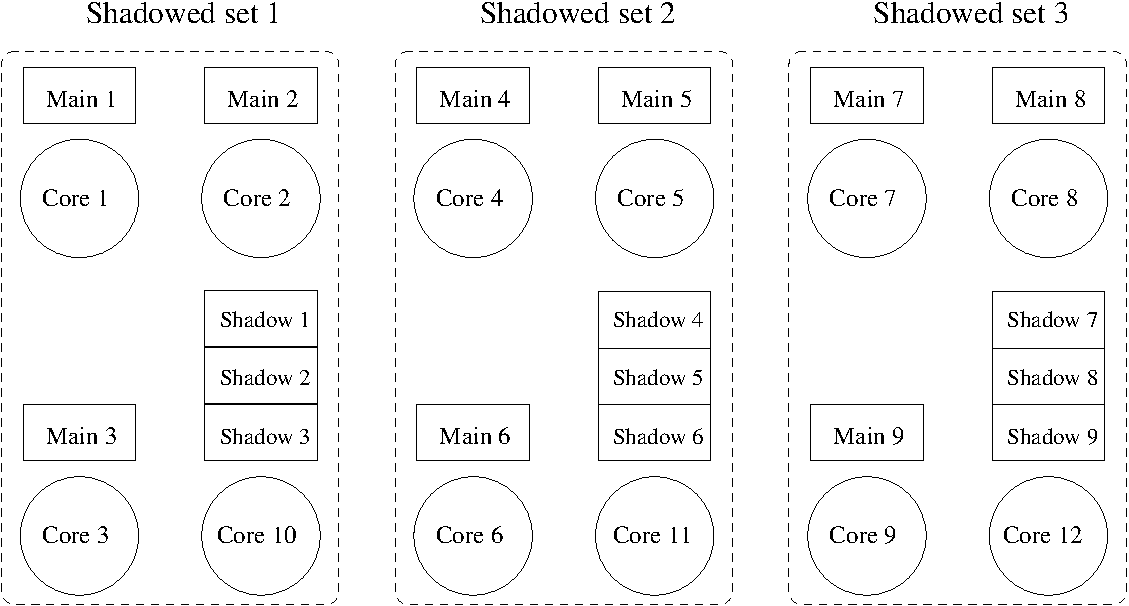
\includegraphics[width=0.6\columnwidth]{Figures/sc_mapping.pdf}
  \end{center}
  %\vskip -0.25in 
  \caption{An example of collocation. $N=12$, $M=9$, $S=3$.}
  \label{fig:sc_mapping}
\end{figure}


\section{Shadow leaping}
\label{sec:leaping_shadows}

As the shadows execute at a lower rate, failures will incur delay for recovery. This problem deteriorates as dependencies incurred by messages and synchronization barriers would propagate the delay of one task to others.  
Fortunately, keeping the mains running at normal rate provides an opportunity for the shadows to benefit from the faster execution of their mains. By copying the state of each main to its shadow, which is similar to the process of storing a checkpoint in a buddy in \cite{zheng_2004_ftccharm}, forward progress is achieved for the shadows with minimized time and energy. This technique, referred to as \textit{shadow leaping}, effectively limits the distance between main and shadow in progress. 
As a result, the recovery time after a failure, which depends on the distance between the failing main 
and its shadow, is also reduced. 
More importantly, 
we opportunistically overlap shadow leaping with failure recovery to avoid extra overhead. 

Assuming a failure occurrence at time $t_f$, Figure~\ref{fig:leap} shows the concept of shadow leaping. 
Upon failure of a main process, its associated shadow speeds up to minimize the impact of failure recovery on the other tasks' progress, as illustrated in Figure~\ref{fig:jump1}. 
At the same time, as shown in Figure~\ref{fig:jump2}, the remaining main processes continue execution until the barrier at $W_{syn}$, and then become idle until $t_r$. 
Shadow leaping opportunistically takes advantage of this idle time to {\it leap forward} the shadows, so that  
all processes, including shadows, can resume execution from a consistent point afterwards. 
Shadow leaping increases the shadow's rate of progress, at a minimal energy cost. Consequently, it reduces significantly the likelihood of a shadow falling excessively behind, thereby ensuring fast recovery while minimizing the total energy consumption.

\begin{figure}[!t]
	\begin{center}
        \subfigure[Faulty task behavior.]
		{
			\label{fig:jump1}
			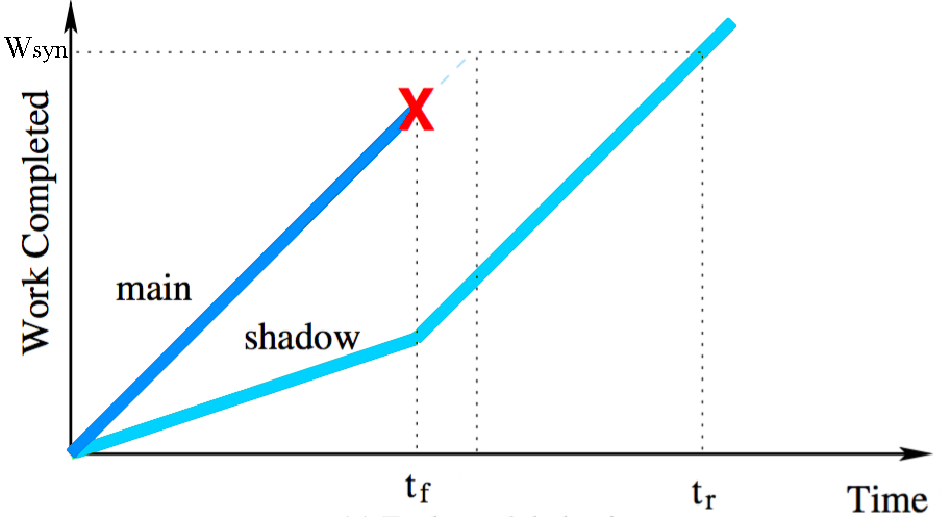
\includegraphics[width=0.4\columnwidth]{Figures/jump1.pdf}
		}
		\subfigure[Non-faulty task behavior.]
		{
			\label{fig:jump2}
			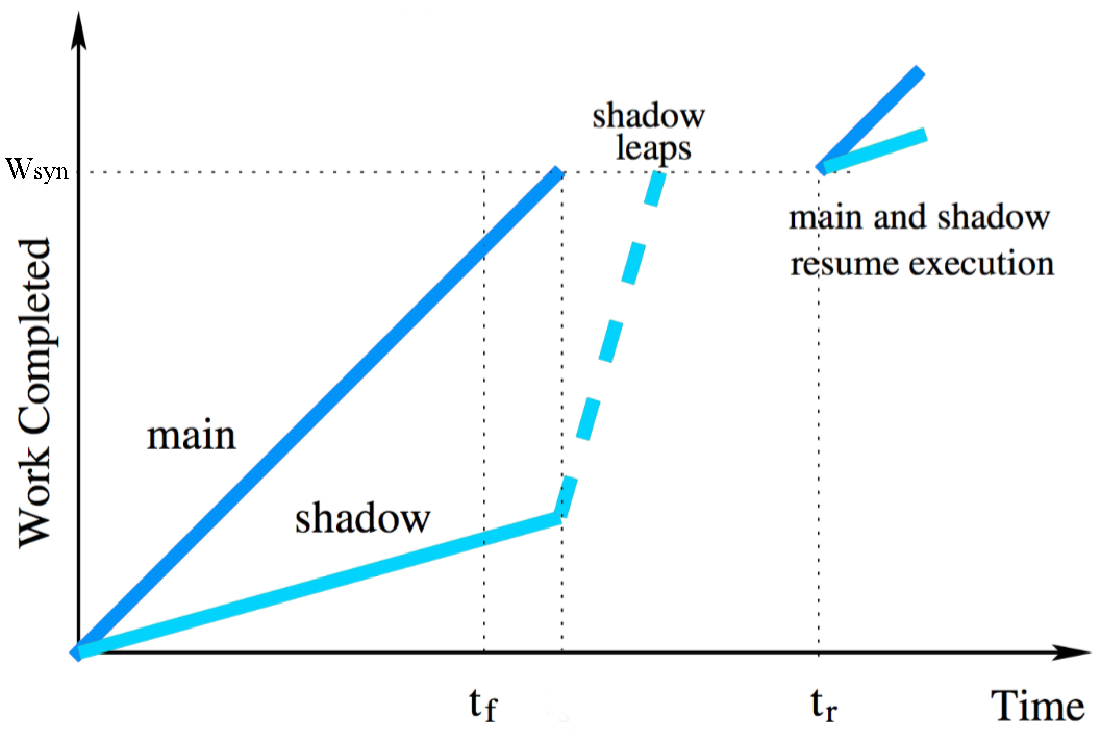
\includegraphics[width=0.4\columnwidth]{Figures/jump2.pdf}
		}
	\end{center}
	\caption{The illustration of shadow leaping.}
	\label{fig:leap}
\end{figure}
\vskip -0.5in
%\section{Analytical framework}
%
%In the following we develop analytical models to quantify the expected performance of Lazy Shadowing, as well as prove the bound on performance loss due to failures. 
%All the analysis below is under the assumption that there are a total of $N$ cores, and $W$ is the application workload.  
%$M$ of the $N$ cores are allocated for main processes, each having a workload of $w=\frac{W}{M}$, and the rest $S$ cores are for the collocated shadow processes. %For process replication,
%Note that process replication is a special case of Lazy Shadowing where $\alpha=1$, so 
%$M=S=\frac{N}{2}$ and $w=\frac{2W}{N}$. 
%
%An application has to roll back when all replicas of a task have been lost. We call this an application fatal failure, which is inevitable even when every process is replicated. 
%In order to take into account the overhead of rollback in the calculation of completion time and energy consumption, we first 
%study the probability of application fatal failure. 
%We use 
%$f(t)$ to denote the failure probability density function of each core, and then $F(t) = \int_0^tf(\tau)d\tau$ is the probability that a core fails in the next $t$ time. 
%Since each shadowed set can tolerate one failure, 
%then the probability that a shadowed set with $\alpha$ main cores and 1 shadow core does not fail by time $t$ is the probability of no failure plus the probability of one failure, i.e., 
%
%\begin{equation}
%	P_g = \Big(1-F(t)\Big)^{\alpha+1} + {{\alpha+1} \choose 1}F(t)\times \Big(1-F(t)\Big)^{\alpha}
%\end{equation}
%and the probability that an fatal failure occurs to an application using $N$ cores within $t$ time is the complement of the probability that
%none of the shadowed sets fails, i.e.,
%
%\begin{equation}
%	P_a = 1 - ({P_g})^{S}
%\end{equation}
%where $S=\frac{N}{\alpha+1}$ is the number of shadowed sets.
%The application fatal failure probability can then be calculated by using $t$ equal to the expected completion time of the application, which will be modeled in the next subsection.
%
%There are two types of delay due to failures. If a failure does not lead to an application fatal failure, the delay corresponds to the catching up of the shadow of the failing main (see Figure~\ref{fig:jump1}). Otherwise, a possible larger (rollback) delay will be introduced by an application fatal failure. In the following we consider both delays step by step. 
%First we discuss the case of $k$ failures without application fatal failure. Should a failure occur during the recovery of a previous failure, its recovery would overlap with the ongoing recovery. To study the worst case behavior, we assume failures do not overlap, so that the execution is split into $k+1$ intervals, as illustrated in Figure~\ref{fig:progress}. 
%$\Delta_i$ ($1\le i \le k+1$) represents the $i^{th}$ execution interval, and $\tau_i$ ($1\le i \le k$) is the recovery time after $\Delta_i$. 
%
%\begin{figure}[!t]
%	\begin{center}
%		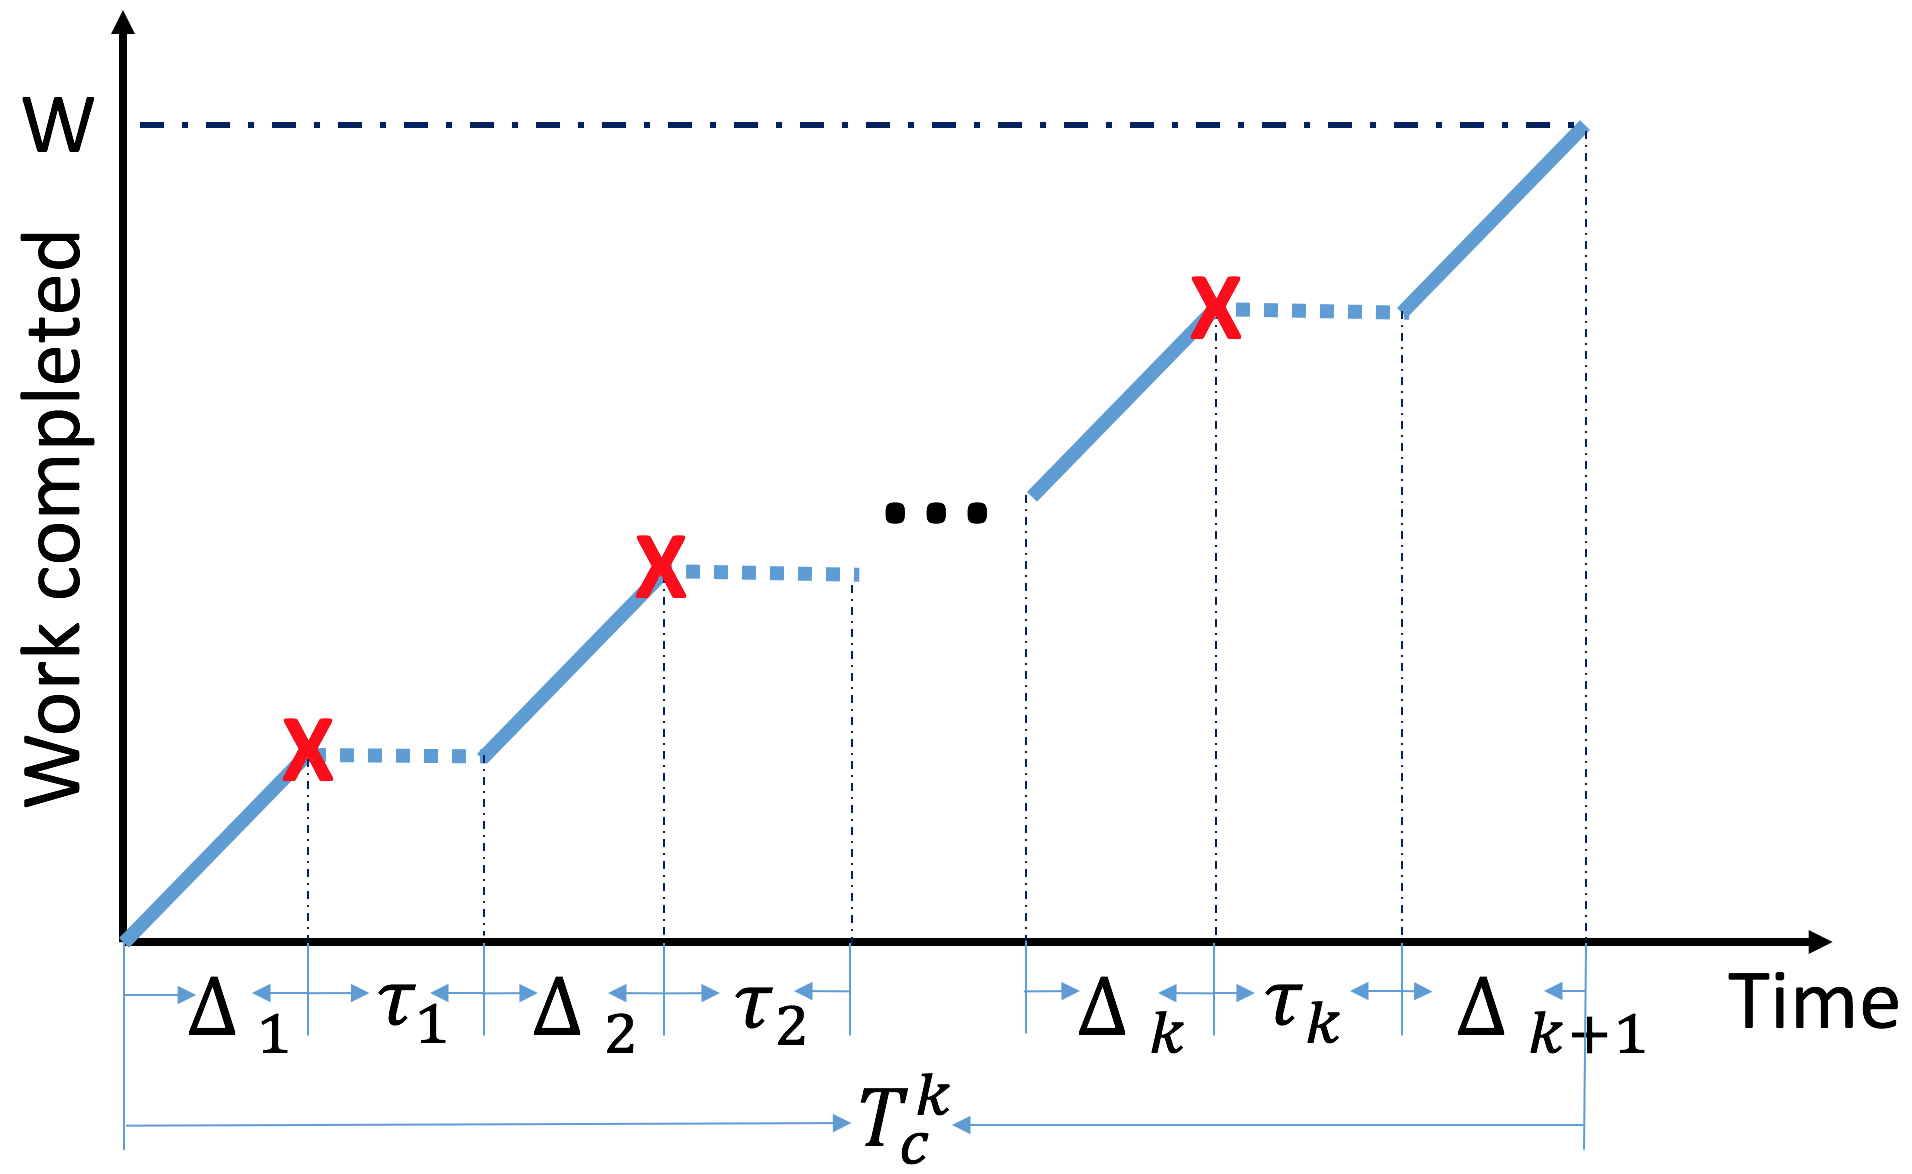
\includegraphics[width=0.7\columnwidth]{Figures/progress}
%	\end{center}
%	%\vskip -0.22in 
%	\caption{Application's progress with shadow catching up delays.}
%	\label{fig:progress}
%\end{figure}
%
%
%The following theorem expresses the completion time, $T_c^k$, as a function of $k$.
%
%\begin{theorem}
%Assuming that failures do not overlap and no application fatal failure occurs, then using Lazy Shadowing, 
%	$$T_c^k = w + (1-\sigma_s^b)\sum_{i=1}^k\Delta_i$$
%\end{theorem}
%\begin{proof}
%
%Lazy Shadowing guarantees that all the shadows reach the same execution point as the mains (See Figure~\ref{fig:leap}) after a previous recovery, so every recovery time is proportional to its previous execution interval. %, which is $\Delta_i$. 
%That is, $\tau_i = \Delta_i \times (1 - \sigma_s^b)$. 
%According to Figure~\ref{fig:progress}, the completion time with $k$ failures is 
%	$T_c^k = \sum_{i=1}^{k+1}\Delta_i + \sum_{i=1}^k\tau_i = w + (1-\sigma_s^b)\sum_{i=1}^k\Delta_i$
%\end{proof}
%
%Although it may seem that the delay would keep growing with the number of failures, 
%it turns out to be well bounded, as a benefit of shadow leaping: 
%
%\begin{corollary}
%The delay induced by failures is bounded by $(1-\sigma_s^b)w$.
%\end{corollary}
%\begin{proof}
%From above theorem we can see the delay from $k$ failures is $(1-\sigma_s^b)\sum_{i=1}^k\Delta_i$. It is straightforward that, for any non-negative integer of $k$, we have the equation $\sum_{i=1}^{k+1}\Delta_i= w$. As a result, 
%$\sum_{i=1}^{k}\Delta_i = w - \Delta_{k+1} \le w$. Therefore, $(1-\sigma_s^b)\sum_{i=1}^k\Delta_i \le (1-\sigma_s^b)w$.
%\end{proof}
%
%Typically, the number of failures to be encountered is stochastic. Given a failure distribution, however, we can calculate the probability for a specific value of $k$. We assume that failures do not occur during recovery, so the failure probability of a core during the execution can be calculated as $P_c = F(w)$. Then the probability that there are $k$ failures among the $N$ cores is 
%\begin{equation}
%\begin{split}
%P_s^{k}= & \dbinom{N}{k}{P_c}^k(1-P_c)^{N-k} \\
%\end{split}
%\end{equation}
%
%The following theorem expresses the expected completion time, $T_{total}$, considering all possible number of failures. 
%
%\begin{theorem}
%Assuming that failures do not overlap, then using Lazy Shadowing,
%$T_{total} = T_{c} / (1 - P_a)$, where $T_{c} = \sum_{i} T_{c}^{i} \cdot P_s^{i}$.
%\end{theorem}
%\begin{proof}
%Without application fatal failure, the completion time considering all possible values of $k$ can be averaged as $T_{c} = \sum_{i} T_{c}^{i} \cdot P_s^{i}$. If an application fatal failure occurs, however, the application needs to roll back to the beginning. With the probability of rollback calculated as $P_a$ in Section~\ref{anal_app_fail}, the total expected completion time is $T_{total} = T_{c} / (1 - P_a)$.
%\end{proof}
%
%Process replication is a special case of Lazy Shadowing where $\alpha=1$, so we can use the above theorem to derive the expected completion time for process replication using the same amount of cores:
%
%\begin{corollary}
%The expected completion time for process replication is $T_{total} = 2W/N / (1 - P_a)$.
%\end{corollary}
%\begin{proof}
%Using process replication, half of the available cores are dedicated to shadows so that the workload assigned to each task is significantly increased, i.e., $w=2W/N$. Different from cases where $\alpha \ge 2$, failures do not incur any delay except for application fatal failures. %, since the replicas are executing at the same rate as the main processes. 
%As a result, without application fatal failure the completion time under process replication is constant regardless of the number of failures, i.e., $T_c=T_c^k=w=2W/N$. Finally, the expected completion time considering the possibility of rollback is $T_{total} = T_c / (1 - P_a) = 2W/N / (1 - P_a)$.
%\end{proof}
%
%Power consumption consists of two parts, dynamic power, $p_d$, which exists only when a core is executing, and static power, $p_s$, which is constant as long as the machine is on. This can be modeled as $p = p_d + p_s$. Note that in addition to CPU leakage, other components, such as memory and disk, also contribute to static power. 
%
%
%For process replication, all cores are running all the time until the application is complete. Therefore, the expected energy consumption, $En$, is proportional to the expected execution time $T_{total}$: 
%\begin{equation}
%%En = N * p * T_{total}
%En = N \times p \times T_{total}
%\label{eq:exp_energy1}
%\end{equation} 
%
%Even using the same amount of cores, Lazy Shadowing can save power and energy, since main cores are idle during the recovery time after each failure, and the shadows can achieve forward progress through shadow leaping. During normal execution, all the cores consume static power as well as dynamic power. During recovery time, however, the main cores are idle and consume only static power, while the shadow cores first perform shadow leaping and then become idle. Altogether, the expected energy consumption for Lazy Shadowing can be modeled as 
%\begin{equation}
%En = N \times p_s \times T_{total} + N \times p_d \times w + S \times p_{l} \times T_l.
%%En = N * p_s * T_{total} + N * p_d * w + S * p_{l} * T_l.
%\label{eq:exp_energy2}
%\end{equation}
%with $p_{l}$ denoting the dynamic power consumption of each core during shadow leaping and $T_l$ the expected total time spent on leaping.

\section{Performance evaluation}
We develop analytical models to quantify
the expected performance of Lazy Shadowing, as well as
prove the bound on performance loss due to failures.
 Please refer to~\cite{cui_2016_scalcom} for details. 
Careful analysis of the models leads us to identify several important factors that determine the performance. These factors can be classified into three categories, i.e., system, application, and algorithm. The system category includes static power ratio $\rho$ ($\rho=p_s/p$), total number of cores $N$, and MTBF of each core; the application category is mainly the total workload, $W$; and shadowing ratio $\alpha$ in the algorithm category determines the number of main cores and shadow cores ($N=M+S$ and $\alpha=M/S$). In this section, we evaluate each performance metric of Lazy Shadowing, 
 %using the models above, 
 with the influence of each of the factors considered.

We compare with both process replication and checkpointing. %, assuming the same number of cores to use. 
The completion time with checkpointing is calculated with Daly's model~\cite{daly_fgcs_2006} assuming 10 minutes for both checkpointing time and restart time. %The energy consumption is then derived with Equation~\ref{eq:exp_energy1}. 
It is important to point out that we always assume the same number of cores available to use, so that process replication and Lazy Shadowing do not use extra cores for the replicas. 

%It is clear from THEOREM 1 that the total recovery delay $\sum_{i=1}^k\tau_i$ is determined by the execution time $\sum_{i=1}^k\Delta_i$, independent of the distribution of failures. 
%% which determines the individual value of $\Delta_i$. 
%Therefore, our models are generic with no assumption about failure probability distribution, and the expectation of the total delay from all failures is the same as if failures are uniformly distributed~\cite{daly_fgcs_2006}. Specifically, $\Delta_i = w/(k+1)$, and $T_c^k = w + w*(1-\sigma_s^b)*\frac{k}{k+1}$. Further, we assume that each shadow gets a fair share of its core's execution rate so that $\sigma_s^b = \frac{1}{\alpha}$.
%To calculate Equation~\ref{eq:exp_energy2}, we assume that the dynamic power during shadow leaping is twice of that during normal execution, i.e., $p_{l}=2*p_d$, and the time for shadow leaping is half of the recovery time, i.e., $T_l=0.5*(T_{total} - w)$ 

The first study uses $N=1$ million cores, %effectively simulating the future extreme-scale computing environment, and assumes that $W=1$ million hours. 
$W=1$ million hours, and static power ratio $\rho=0.5$.
Our results show that at extreme-scale, the completion time and energy consumption of checkpointing are orders of magnitude larger than those of Lazy Shadowing and process replication. Thus, we choose not to plot a separate graph for checkpointing in the interest of space. 
Figure~\ref{fig:t32} reveals that the most time efficient choice largely depends on MTBF. 
%More specifically, process replication consumes less time when MTBF is low while otherwise Lazy Shadowing is more efficient.
When MTBF is high, Lazy Shadowing requires less time as more cores are used for main processes and less workload is assigned to each process. As MTBF decreases, process replication outperforms Lazy Shadowing as a result of the increased likelihood of rollback for Lazy Shadowing.
In terms of energy consumption, Lazy Shadowing has a much larger advantage over process replication. %For MTBF from 2 to 25 years, Lazy Shadowing with $\alpha=5$ can achieve 9.6-17.1\% energy saving, while the saving increases to 13.1- 23.3\% for $\alpha=10$. The only exception is when MTBF is extremely low (1 year), Lazy Shadowing with $\alpha=10$ consumes more energy because of extended execution time.

\begin{figure}[!t]
	%\captionsetup{justification=centering}
	\begin{center} 
		\subfigure[Expected completion time]
		{
			\label{fig:t32}
			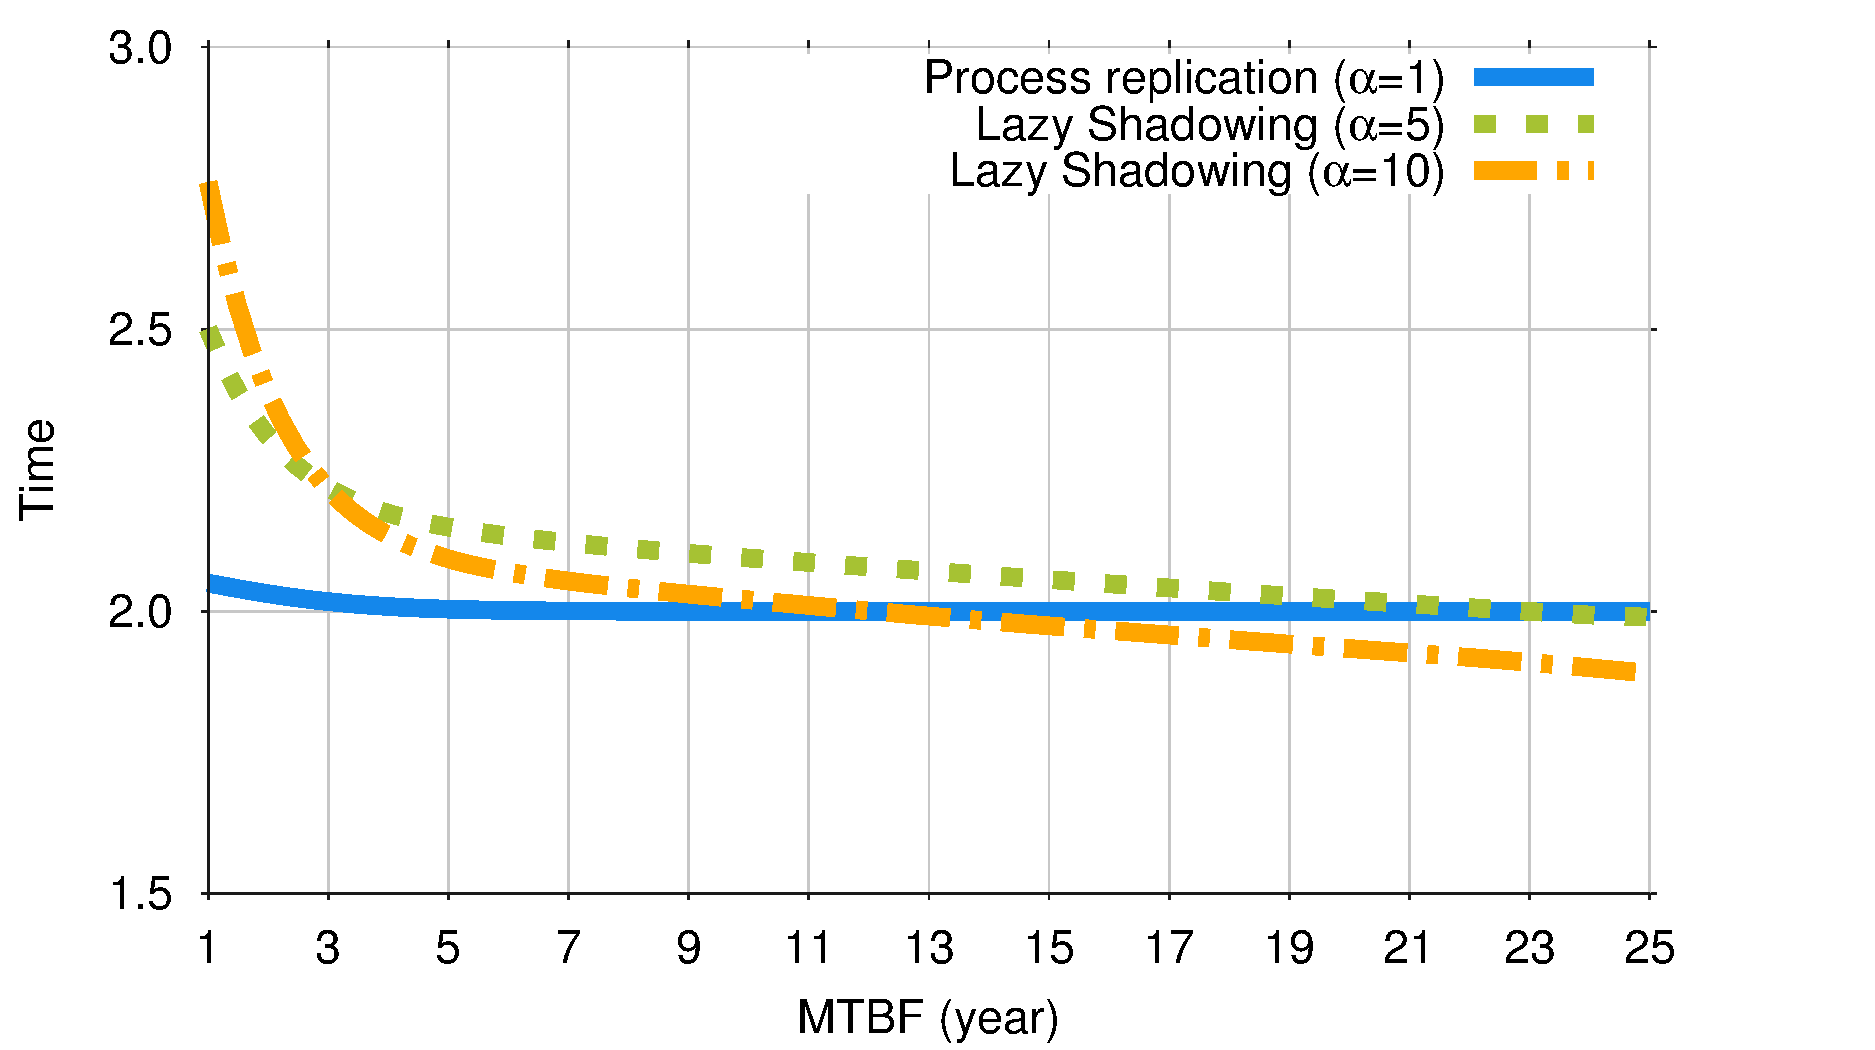
\includegraphics[width=0.4\columnwidth]{Figures/gen_time.pdf}
			%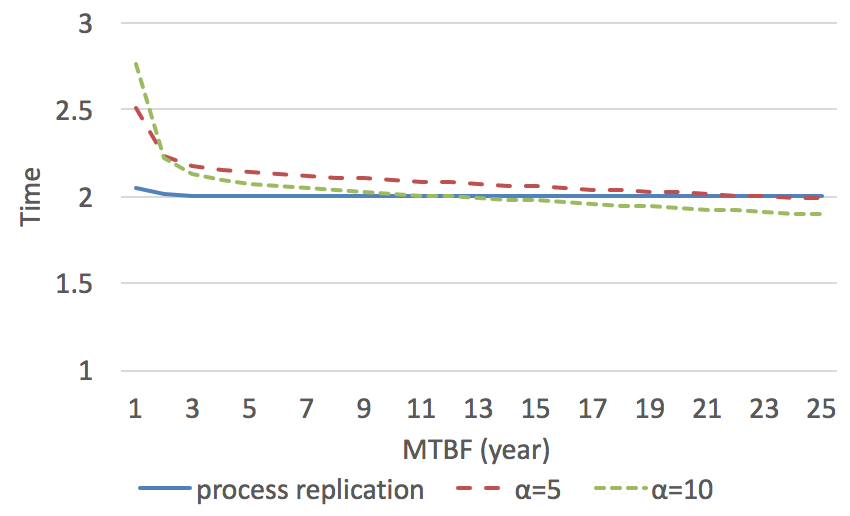
\includegraphics[width=0.7\columnwidth]{Figures/tt32}
		} 
		\subfigure[Expected energy consumption]
		{
			\label{fig:e32}
			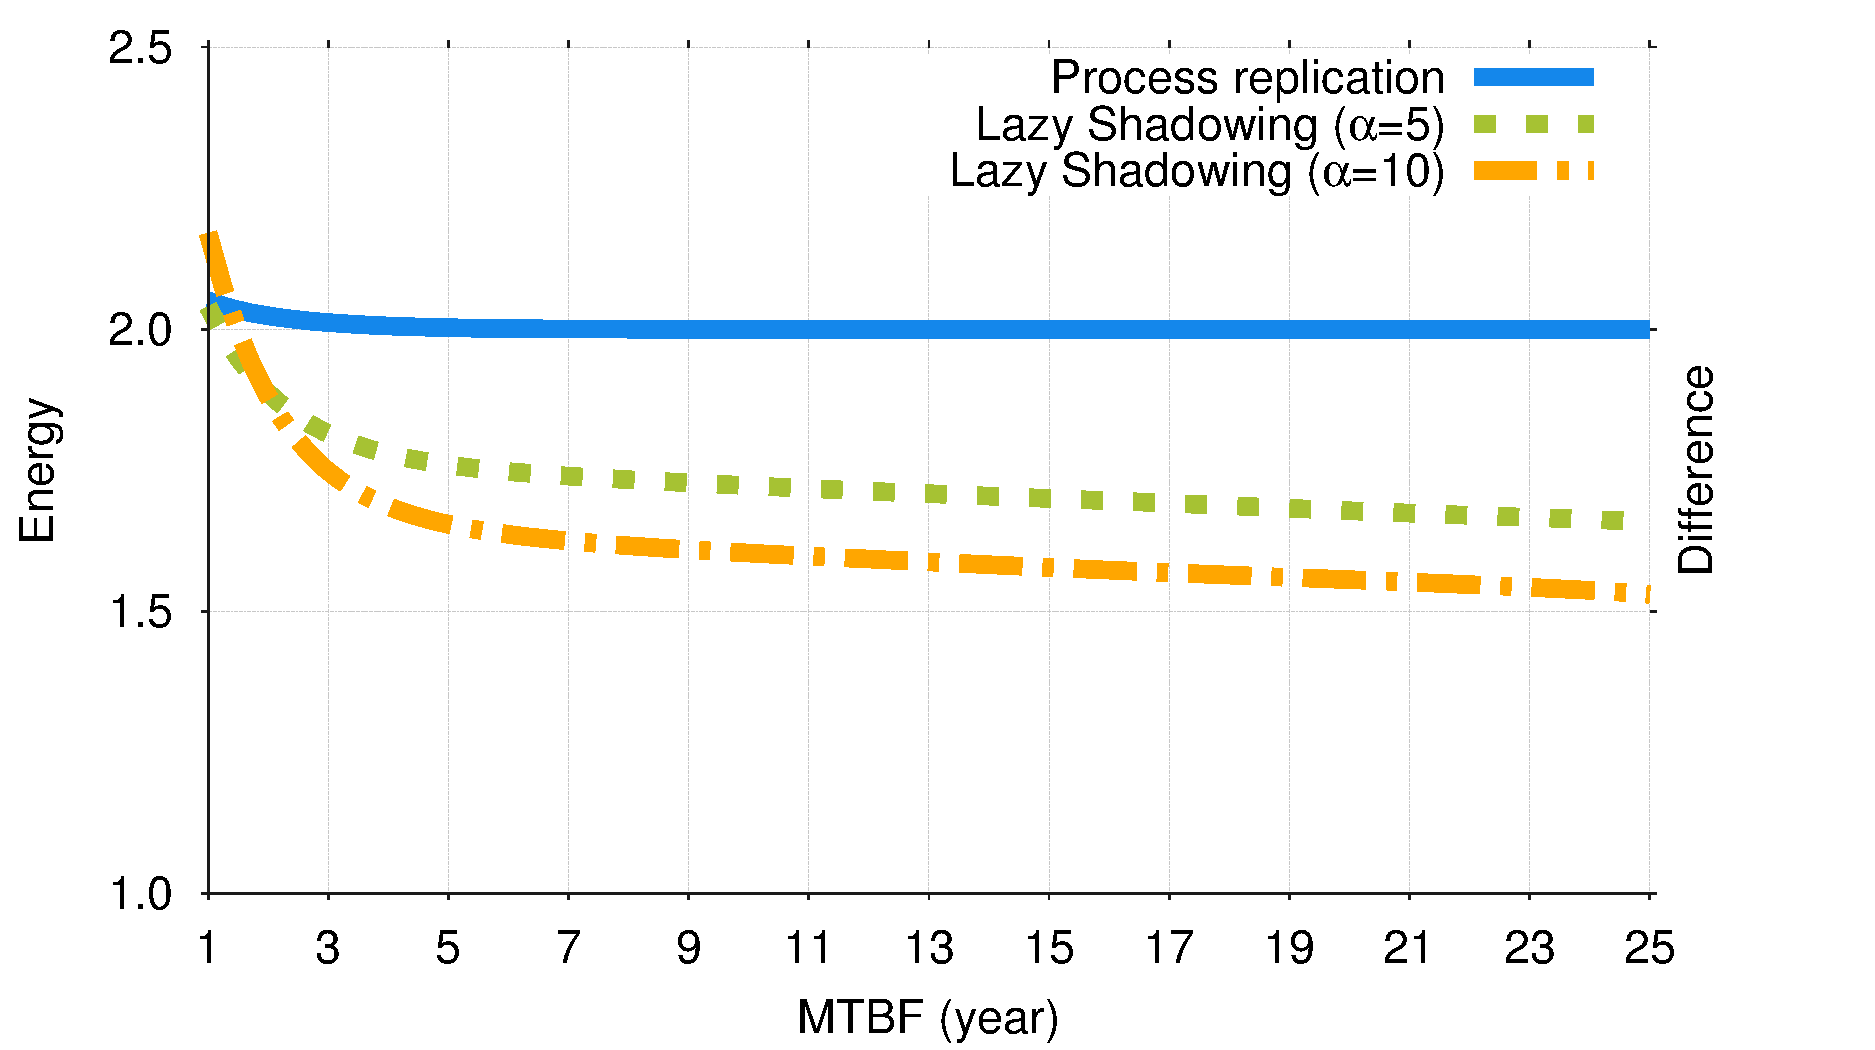
\includegraphics[width=0.4\columnwidth]{Figures/gen_energy.pdf}
			%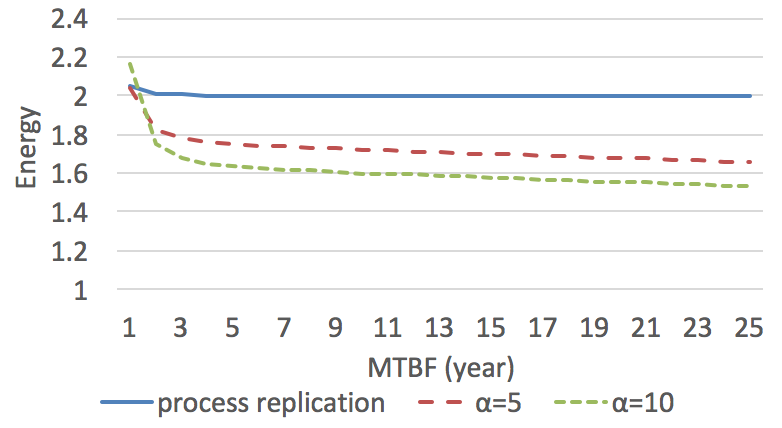
\includegraphics[width=0.7\columnwidth]{Figures/te32}
		} 
		\caption{Comparison of time and energy for different core level MTBF. $W=10^6$ hours, $N=10^6$, $\rho=0.5$.}
	\end{center}
	%\vskip -0.22in 
	\label{fig:com3}
\end{figure}

The system scale, measured in number of cores, has a direct impact on the failure rate seen by the application. To study its impact, we vary $N$ from 10,000 to 1,000,000 with $W$ scaled proportionally, i.e., $W=N$. When MTBF is 5 years, the results are shown in Figure~\ref{fig:n5}. Please note that the time and energy for checkpointing when $N=1,000,000$ are beyond the scope of the figures, so we mark their values on top of their columns. When completion time is considered, Figure~\ref{fig:nt5} clearly shows that each of the three fault tolerance alternatives has its own advantage. %Specifically, checkpointing is the best choice for small systems at the scale of 10,000 cores, Lazy Shadowing outperforms others for systems with 100,000 cores, while process replication has slight advantage over Lazy Shadowing for larger systems. 
On the other hand, Lazy Shadowing wins for all system sizes when energy consumption is the objective. 

%When MTBF is changed to 25 years, the performance of checkpointing improves a lot, but is still much worse than that of the other two approaches. Lazy Shadowing benefits much more than process replication from the increased MTBF. As a result, Lazy Shadowing is able to achieve shorter completion time than process replication when $N$ reaches 1,000,000.

\begin{figure}[!t]
	%\captionsetup{justification=centering}
	\begin{center}
		\subfigure[Expected completion time]
		{
			\label{fig:nt5}
			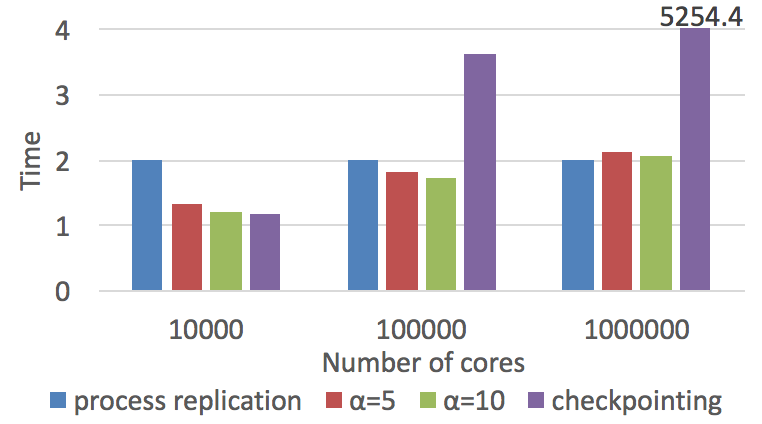
\includegraphics[width=0.4\columnwidth]{Figures/tnt5}
		} 
		\subfigure[Expected energy consumption]
		{
			\label{fig:ne5}
			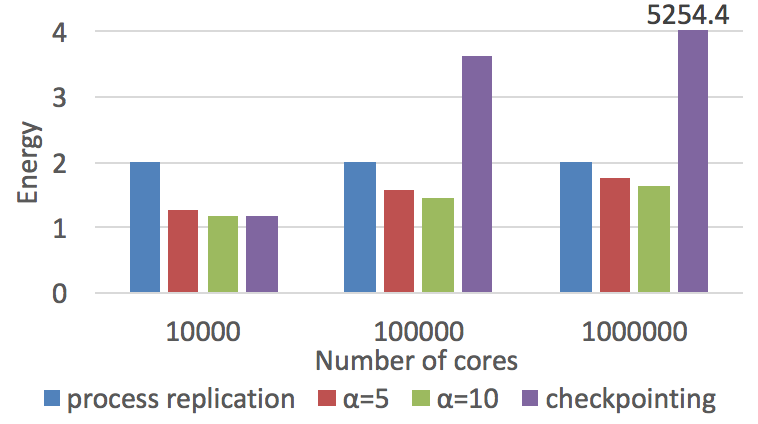
\includegraphics[width=0.4\columnwidth]{Figures/tne5}
		} 
	\end{center}
	%\vskip -0.22in 
	\caption{Comparison of time and energy for different number of cores. $W=N$, MTBF=5 years, $\rho=0.5$.}
	\label{fig:n5}
\end{figure}

With various architectures and organizations, servers
vary in terms of
power consumption. The static power ratio $\rho$ is used to abstract the
amount of static power consumed versus dynamic power. 
%$\rho$ does not impact the completion time, but power and energy consumption.
Considering modern systems, we vary $\rho$ from 0.3 to 0.7 and study its effect
on the expected energy consumption. The results for Lazy Shadowing with $\alpha=5$ are normalized to that of process replication and shown in 
Figure~\ref{fig:power_ratio}. 
%The results for other values of $\alpha$ have similar behavior and thus are not shown. 
Lazy Shadowing achieves
more energy saving when the static power ratio is low, since it saves dynamic 
power but not static power. %When static power ratio is low ($\rho=0.3$), Lazy Shadowing
%is able to save 20\%-24\% energy for the MTBF of 5 to 25 years. The saving decreases to 5\%-11\% when $\rho$ reaches 0.7. 

\begin{figure}[!t]
	%\captionsetup{justification=centering}
	\begin{center}
		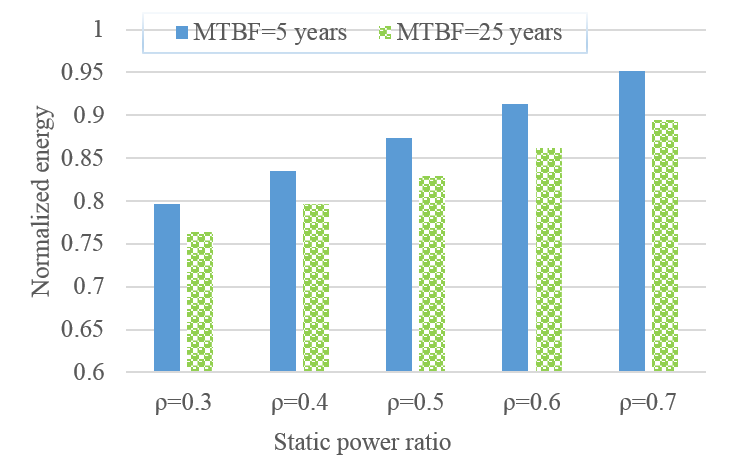
\includegraphics[width=0.7\columnwidth]{Figures/ts_power_5}
	\end{center}
	%\vskip -0.22in 
	\caption{Impact of static power ratio on energy consumption. $W=10^6$ hours, $N=10^6$, $\alpha$=5.}
	\label{fig:power_ratio}
\end{figure}

\section{Summary}

%As the scale and complexity of HPC systems continue to increase, both the failure rate and power consumption are expected to increase dramatically, making it extremely challenging to deliver extreme-scale computing performance efficiently. Existing fault tolerance methods rely on either time or hardware redundancy. Neither of them appeals to the next generation of supercomputing, as the first approach may incur significant delay while the second one constantly wastes over 50\% of the system resources.

In this work, we present a comprehensive discussion of the techniques that enable Lazy Shadowing to achieve scalable resilience in future extreme-scale computing systems. In addition, we develop a series of analytical models to assess its performance in terms of reliability, completion time, and energy consumption. 
Through comparison with existing fault tolerance approaches, we identify the scenarios where each of the alternatives should be chosen for best performance.












\chapter{lsMPI: an implementation in MPI}
\label{chapter:implementation}
In a complex system like what we have today, the behavior of Lazy Shadowing is subject to both the hardware configuration, such as failure detection and execution rate control, and software behavior, such as the amount of communication and synchronization. 
It's difficult for an analytical framework to precisely capture every details of Lazy Shadowing when it runs in a real environment. Therefore, a functional prototype is necessary to prove its validity as well as measure its actual performance. 

We are implementing Lazy Shadowing as a library (lsMPI) for MPI, which is the de facto programming paradigm for HPC. Instead of a full-feature MPI implementation, the library is designed to be a separate layer between MPI and user application, and uses the MPI profiling hooks to intercept every MPI call. There are three benefits for this choice: 1) we can save tremendous time and efforts of rebuilding MPI from scratch; 2) we can take advantage of existing MPI performance optimizations that numerous researches have spent years on; and 3) the library is portable across all MPI implementations. 
The library will spawn the shadow processes at initialization phase, manage the coordination between main and shadow processes during execution, and guarantee order and consistency for messages and non-deterministic events.
Once completed, users should be able to link to the library without any change to existing code. 

Same as rMPI~\cite{ferreira_sc_2011}, lsMPI uses the underlying Reliability, Availability and Serviceability (RAS) system to detect process failure. In this prototype system, we will emulate a RAS system at the user level, and use an event mechanism to inform lsMPI whenever RAS detects a failure. When initializing, each process installs a signal handler dedicated for failure detection and notification. When a process is about the fail, RAS will send a signal to the process and triger the handler, which forces the process to fail and use out-of-band messages to notify other processes of the failure. 

When user specifies $N$ processes, we will transparently translate it into $2N + K$ processes where $K$ is the number of shadowed sets. In our wrapper of MPI_Init() we will spawn $N$ main processes, $N$ shadow processes, and $K$ shadow coordinators. User has the flexibility to specify how the main processes are orgnanized into shadowed sets through a rankfile. With a rankfile as input, lsMPI creates a process as shadow coordinator for each shadowed set. The logical organization is depicted in Figure~\ref{fig:logical_org}. 

\begin{figure}[!t]
  \begin{center}
      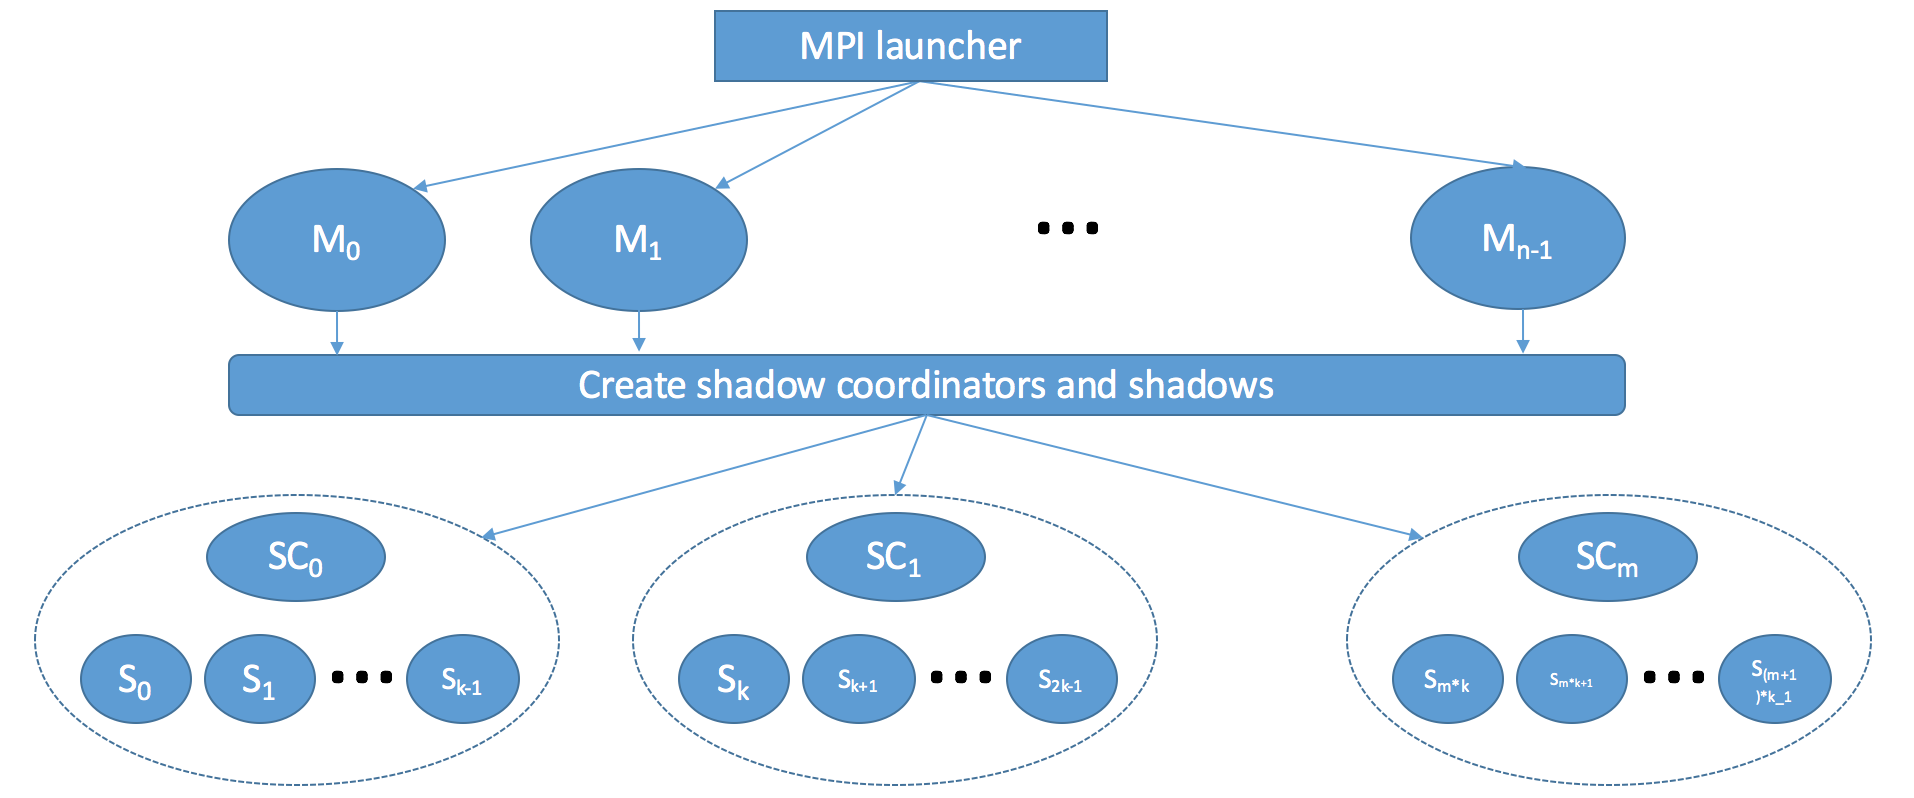
\includegraphics[width=0.7\columnwidth]{figures/logical_org}
  \end{center}
  \caption{Logical organization of a MPI world with Lazy Shadowing.}
  \label{fig:logical_con}
\end{figure}

State consistency is required both during normal execution and following a failure. % of a main process to roll-forward the shadows. 
We design a consistency protocol as shown in Figure~\ref{fig:cons_protocol}, 
to assure 
that the shadows see the same message order and MPI operation results as the mains. In this figure, A and B represent two mains, and A' and B' are their shadows. 
For each message, the main of the sender sends a copy of the message to each of the main and shadow of the receiver, and the shadow of the sender is suppressed from sending out messages until its main process fails. %After sending out the message, the main sends an ACK to its shadow, so that the shadow can safely suppress sending the message and proceed. 
If a main fails,
its associated shadow will become a new main. Same as the previous main, the new main sends 2 copies for each application message. 
To assure consistent transition, i.e., there is neither duplicate or missing message, we require the main to send a ACK after each application message. With ACKs, the shadow knows exactly which messages have been sent out before its main fails. 


\begin{figure}[!t]
  \begin{center}
  	\subfigure[Before failure]
		{
			\label{fig:consist_w_fail}
      		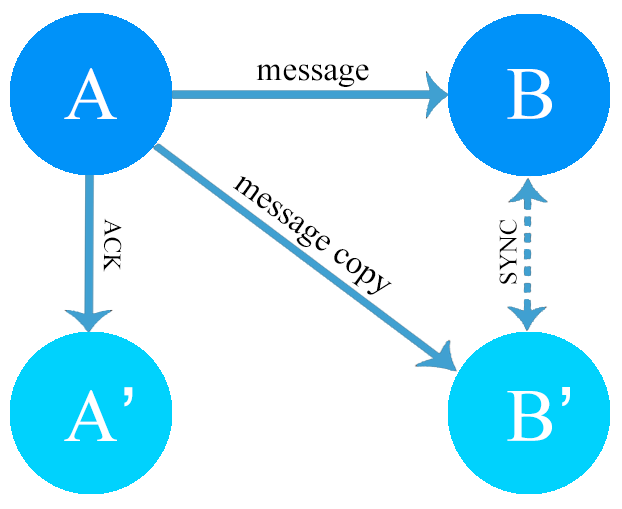
\includegraphics[width=0.4\columnwidth]{figures/cons_protocol}
      	}
  	\subfigure[After failure]
		{
			\label{fig:consist_wo_fail}
      		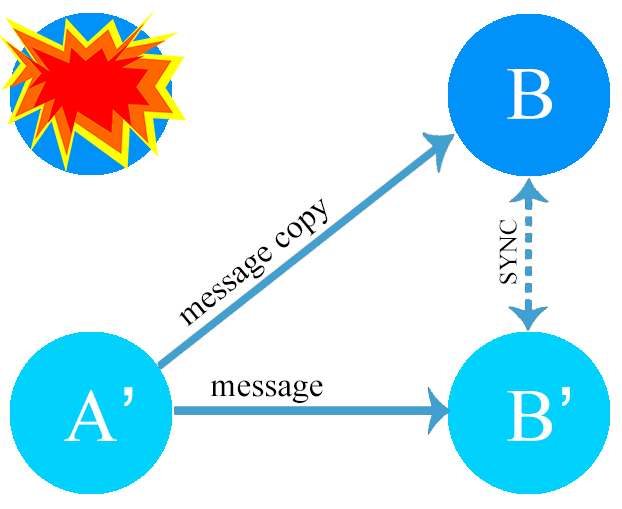
\includegraphics[width=0.4\columnwidth]{figures/cons_protocol_failure.png}
      	}
  \end{center}
  %\vskip -0.25in
  \caption{Consistency protocol for lsMPI.}
  \label{fig:cons_protocol}
\end{figure}

We assume that only MPI operations can introduce non-determinism. MPI\_ANY\_SOURCE receives may result in different message orders between the main and shadow. To deal with this, we always let the main receive a message ahead of the shadow and then forward the message source to its shadow (SYNC message in Figure~\ref{fig:cons_protocol}). 
The shadow then issues a receive with the specific source. Other operations, such as MPI\_Wtime() and MPI\_Probe(), can be dealt with by always forwarding the result from the main to the shadow.

Remote Direct Memory Access (RDMA) will be used to leap forward the state of the shadow to be consistent with that of its associated main. Rather than copying data to the buffers of the OS, RDMA allows to transfer data directly from the main process to its shadow. The zero-copy feature of RDMA considerably reduces latency, thereby enabling fast transfer of data between the main and its shadow.

\chapter{Smart shadowing}
\label{chapter:smart}
In the most general form of Lazy Shadowing, each main is associated with one shadow that executes the same workload. This is ignorant of the variance in the underlying hardware reliability and above application criticality.

\chapter{TIMELINE OF PROPOSED WORK}
\label{chapter:timeline}
\begin{table}[ht]
\vspace{-0.3in}
\caption{Timeline of Proposed Work.}
\vspace{-0.15in}
\centering
\scalebox{0.85}
{
\begin{tabular}{|l|l|l|}
\hline
\textbf{Date} & \textbf{Content} & \textbf{Deliverable results} \\
\hline
Jan - Feb  & Explore restoring in approximate computing & Pin-based framework for \\
 & in Section \ref{work:approx} of Chapter \ref{chapter:future_study}& restoring approximation \\
\hline
Mar - May  & Integrate restoring with information leakage & Experimental data of memory\\% through access pattern &  Paper submission \\
 & in Section \ref{work:security} of Chapter \ref{chapter:future_study}& performance and security\\
\hline
Jun - Sep & Study restoring in Hybrid Memory Cube (HMC) & Modified simulator of temperature\\
 & in Section \ref{work:stacked} of Chapter \ref{chapter:future_study}&  effect of restoring in HMC \\
\hline
Jul - Oct  & Thesis writing & Thesis ready for defense \\
\hline
Oct - Dec & Thesis revising & Completed thesis \\
\hline
\end{tabular}
}
\label{tab:timeline}
\end{table}

The proposed works will be undertaken as shown in the Table \ref{tab:timeline}.
I will start the effort with task (1) to develop Pin-based framework for approximate computing of restoring. This task involves program annotation, chip generation, QoS evaluation, and conventional performance simulation, etc.
While multiple complicated subtasks are there, this task has been partially finished, and will not take much time to complete.
Afterwards, I'll move to task (2) to study information leakage in restoring scenario, and this task is partially on basis of the previous approximation work.
With the completion of task (2), the overall goal of exploring DRAM restoring in application level have been reached, and then I'll start the study restoring's temperature effect in HMC, i.e., task (3).
The general infrastructure can be borrowed from my previous HMC work \cite{ICCD15:dlb}. This task might be performed concurrently with other jobs, and thus might take more time to finish.
At the end of task (3), the holistic exploration of DRAM restoring is considered finished, and thus I'll summarize all the tasks into my final thesis.

\chapter{SUMMARY}
\label{chapter:summary}
\begin{table}[ht]
\vspace{-0.3in}
\caption{Timeline of Proposed Work.}
\vspace{-0.15in}
\centering
\scalebox{0.85}
{
\begin{tabular}{|l|l|l|}
\hline
\textbf{Date} & \textbf{Content} & \textbf{Deliverable results} \\
\hline
Sep.-   & Explore restoring in approximate computing & Pin-based framework for \\
 & in Section \ref{work:approx} of Chapter \ref{chapter:future_study}& restoring approximation \\
\hline
Mar - May  & Integrate restoring with information leakage & Experimental data of memory\\% through access pattern &  Paper submission \\
 & in Section \ref{work:security} of Chapter \ref{chapter:future_study}& performance and security\\
\hline
Jun - Sep & Study restoring in Hybrid Memory Cube (HMC) & Modified simulator of temperature\\
 & in Section \ref{work:stacked} of Chapter \ref{chapter:future_study}&  effect of restoring in HMC \\
\hline
Jul - Oct  & Thesis writing & Thesis ready for defense \\
\hline
Oct - Dec & Thesis revising & Completed thesis \\
\hline
\end{tabular}
}
\label{tab:timeline}
\end{table}





Current fault tolerance approaches rely exclusively on either time or hardware redundancy to hide failures from being seen by users. 
Rollback recovery, which exploits time redundancy, requires full or partial re-execution when failure occurs.  
Such an approach
can incur a significant delay, % subjecting cloud service providers to SLA violations,
and high power costs due to extended execution time.
On the other hand, Process Replication relies on hardware redundancy and executes multiple
instances of the same task in parallel to guarantee completion with minimal delay. 
This solution, however, requires a significant increase in hardware resources and increases the power consumption proportionally. 


\appendix                      
%After this command, chapters will be formatted as appendices. For example
%\chapter{Possible Appendix}
%\label{appendix:effectEventInferenceRules}
%\input{appendixEffectEventInference}

%\chapter*{BIB}
\begin{singlespace}
%\nocite{*}
%\renewcommand{\bibsection}{} %remove automatically generated title, like "REFERENCE" or "BIBLIGROPHY"
\bibliographystyle{plainnat}
{
\footnotesize
\bibliography{proposal}
}
\end{singlespace}
%\bibliography{gfbf,sentiment,agreementStudy,effectEventCorpus,effectEventInference,generalEventCorpus,generalEventInference,myWork}          %\safebibliography is used the same way as \bibliography, but gives pittetd
%                                   a greater chance to succeed in formatting the bibliography when nonstandard
%                                   BibTeX styles are used.
\end{document}
